\RequirePackage{silence}
\WarningFilter{latexfont}{Font shape `TU/}
\WarningFilter{latexfont}{Size substitutions}
\RequirePackage[warnings-off={mathtools-colon,mathtools-overbracket}]{unicode-math}
% Ошибки ^
\documentclass[fleqn]{article}
\usepackage{amsmath,nccmath} % Математика
\usepackage[a5paper, margin=12mm]{geometry}
% Пакеты
\usepackage{polyglossia} % Язык
\setmainlanguage{russian}
\setotherlanguage{english}
\setkeys{russian}{babelshorthands=true}
\usepackage{fontspec} % Шрифты .otf
\usepackage{titlesec} % Заголовки
\usepackage{tabularx,multicol,multirow,array,makecell} % Таблицы
\usepackage{enumitem} % Списки
\usepackage{graphicx,float} % Графика
\usepackage{xcolor} % Цвет
\usepackage{empheq}
\usepackage[makeroom]{cancel}
\usepackage[most]{tcolorbox} % Удобные рамки
\usepackage[open,openlevel=1]{bookmark} % Секции в pdf-файле
\graphicspath{{svg/}}
% Нумерация
\pagenumbering{gobble} % Страницы
\setcounter{secnumdepth}{0} % Заголовки
% Шрифты
\setmainfont[SizeFeatures={Size=12}]{Century Schoolbook}
\setmathfont[Scale=1.2]{TeX Gyre Schola Math}
\newfontfamily\bold[SizeFeatures={Size=12}]{Century Schoolbook Bold}
\newfontfamily\ital[SizeFeatures={Size=12}]{Century Schoolbook Italic}
\newfontfamily\boldital[SizeFeatures={Size=12}]{Century Schoolbook Bold Italic}
\newfontfamily\gilroysub[SizeFeatures={Size=16},UprightFont={*-Medium}]{Gilroy}
\newfontfamily\gilroy[SizeFeatures={Size=19},UprightFont={*-UltraLight}]{Gilroy}
\newfontfamily\tinyt[SizeFeatures={Size=10}]{Century Schoolbook}
% Стили
\titleformat*{\subsection}{\raggedright\gilroysub}
\titleformat*{\section}{\gilroy\centering}
\titlespacing*{\subsection}{0pt}{6pt}{0pt}
\titlespacing*{\section}{0pt}{6pt}{1pt}
\definecolor{desc}{HTML}{888888}
\definecolor{table}{HTML}{D9D9D9}
\newcommand{\modb}[1]{\ \left(\mathrm{mod}\ #1\right)}
\newcommand{\modn}[1]{\ \mathrm{mod}\ #1}
\newcommand{\qedb}{\ \char"25A0}
\newcommand{\qedw}{\ \char"25A1}
\newcommand{\id}[1]{\text{id}_{#1}}
\newcommand{\norm}[1]{\lVert#1\rVert}
\newcommand{\abs}[1]{\left|#1\right|}
\newcommand{\sgnb}[1]{\text{sgn}\hspace*{-2pt}\left(#1\right)}
\newcommand{\sgnn}[1]{\text{sgn}\ #1}
\newcommand{\ren}[1]{\Re\text{e}\ #1}
\newcommand{\reb}[1]{\Re\text{e}\left(#1\right)}
\newcommand{\imn}[1]{\Im\text{m}\ #1}
\newcommand{\imb}[1]{\Im\text{m}\left(#1\right)}
\newcommand{\optm}[1]{\underset{\scriptscriptstyle #1}{\text{opt}}}
\newcommand{\optl}[1]{\text{opt}_{#1}}
\newcommand{\diff}{\text{d}}
\newcommand{\footnotes}[2]{$^{#1}$\hspace*{-1.1pt}\let\thefootnote\relax\footnote
{\hspace*{-18pt}#1 #2}}
\newcommand{\multiset}[2]{\left(\!\!\binom{#1}{#2}\!\!\right)}
\newcommand{\stirl}{\genfrac\{\}{0pt}{}}

% Смена шрифта для \mathcal
\DeclareMathAlphabet{\mathcal}{OMS}{cmsy}{m}{n}
\SetMathAlphabet{\mathcal}{bold}{OMS}{cmsy}{b}{n}

% Понижает высоту степени тригонометрических функций
\newcommand{\trsp}{\hspace*{-2.3pt}\phantom{}}

% Minipage environment
\newenvironment{column*}[2]{
\begin{minipage}[#1]{#2}
\setlength\baselineskip{13.4pt} % Строка
\setlength{\parskip}{6pt} % Абзац
\abovedisplayskip=6pt % Формула над
\belowdisplayskip=6pt % Формула под
\raggedright % Выравнивание
}{\end{minipage}}

% Tabular environment
\def\center{c}

\newenvironment{tabularc}[4]{
\if\center #4
\centering
\fi
\setlength\tabcolsep{#1}
\setlength\extrarowheight{#2}
\begin{tabular}{#3}
}{\end{tabular}\par}

% Tabularx environment
\newenvironment{tabularcx}[4]{
\setlength\tabcolsep{#1}
\setlength\extrarowheight{#2}
\tabularx{#4}{#3}
}{\endtabularx\par}

\newcolumntype{L}{>{\raggedright\arraybackslash}X}
\newcolumntype{R}{>{\raggedleft\arraybackslash}X}
\newcolumntype{C}{>{\centering\arraybackslash}X}

% Square cases environment
\makeatletter\newenvironment{sqcases}{%
  \matrix@check\sqcases\env@sqcases
}{%
  \endarray\right.%
}
\def\env@sqcases{%
  \let\@ifnextchar\new@ifnextchar
  \left\lbrack
  \def\arraystretch{1.2}%
  \array{@{}l@{\quad}l@{}}%
}\makeatother

% Theorem Tcolorbox
\newtcolorbox{theorem}{
enhanced,
boxrule=0mm,frame hidden,arc=0mm,
colback=white!0,
boxsep=0mm,left=3.5mm,
borderline west={2pt}{0pt}{black},
before skip=6pt,after skip=7pt
}


\begin{document}
\raggedright % Выравнивание
\columnsep=6mm % Колонка
\setlength\multicolsep{6pt} % Колонка
\setlength{\baselineskip}{13.4pt} % Строка
\setlength{\parskip}{6pt} % Абзац
\abovedisplayskip=6pt % Формула над
\belowdisplayskip=6pt % Формула под
\setlist[itemize]{nosep,noitemsep} % Список
% Отступы ^

% Rearrange subsections (Алгоритм Евклида)

\section{Элементарная алгебра}

% Вспомнить о понятии окрестности точки,
% функции расстояния --- метрики (см. п. 5)

\subsection{Виды выражений}

{\ital Одночлен \color{desc}(моном)} --- произведение переменных и коэффи"=циентов; {\ital многочлен \color{desc}(полином)} --- сумма одночленов.

{\ital Двучлен \color{desc}(бином)} --- многочлен из двух одночленов; {\ital трёхчлен {\color{desc}(трином)}} --- многочлен из трёх одночленов.

Многочлен $P$ от одной переменной $x$ можно представить так:
% ---
$$P=\sum^{n}_{k=0}a_kx^{n-k}$$

\subsection{Малая теорема Безу}

Для многочлена $P=:P(x)$ справедливо:
% ---
$$P(x)=f(x)(x-r)+P(r)$$
% ---
Это следует из деления многочлена с остатком. Значит,
% ---
$$(x-r)\mid P(x)\iff P(r)=0.$$

\subsection{Свойства неравенств}

Отношение сравнения {\ital транзитивно}; неравенства можно {\ital складывать}
{\ital\color{desc}(не вычитать)}, а также {\ital перемножать} и возво"=дить
в натуральную степень $k$ {\ital\color{desc}(без смены знака)}:
% ---
$$
\begin{cases}
a\less b\\
c\leq d
\end{cases}\hspace*{-12pt}\implies
\begin{cases}
a + c\less b + d\\
ac\less bd\\
a^k\less b^k
\end{cases}
$$
% ---
При умножении на отрицательное число знак неравенства {\ital инвертируется}:
% ---
$$a\less b\iff am\greater bm,\quad m\in\mathbb{R}^-$$

\subsection{Неравенство Коши}

Пусть $a,b\in \mathbb{R}^+$. Тогда верно {\ital\color{desc}(О.Л. Коши)}:
% ---
$$\frac{a+b}{2}\geq \sqrt{ab}$$
% ---
{\bold Доказательство.}
$$\frac{a+b}{2}\geq \sqrt{ab}\iff a+b\geq 2\sqrt{ab}\iff a-2\sqrt{ab}+b\geq 0\iff$$
\\[-11pt]
$$(\sqrt{a}-\sqrt{b})^2\geq 0\qedb$$

\subsection{Неравенство Бернулли}

Пусть $n\geq 2,\ x\greater 0$. Тогда верно {\ital\color{desc}(Я. Бернулли)}:
% ---
$$(1+x)^n\greater 1+nx$$
% ---
{\bold Доказательство.} Проверим базис индукции $n=2$:
% ---
$$(1+x)^2\greater 1+2x\iff 1+2x+x^2\greater 1+2x\qedw$$
% ---
Проверим индукционный шаг $n+1$. Пусть утверждение верно для некоторого
$n\greater 2$, тогда:
% ---
$$(1+x)^n\greater 1+nx\iff (1+x)^{n+1}\greater (1+nx)(1+x)\iff$$
$$(1+x)^{n+1}\greater 1+(n+1)x+nx^2\iff (1+x)^{n+1}\greater 1+(n+1)x\qedb$$

\subsection{Свойства функций}

Функция $f$ {\ital возрастает}, когда
% ---
$$\forall x_1,x_2\in D_f,\ x_1\less x_2\implies f(x_1)\less f(x_2).$$
% ---
{\ital Максимумом} функции $f$ называется такая точка $x_0$, что
% ---
$$\forall\varepsilon\greater 0\ \exists U_\varepsilon(x_0)\colon\forall x\in U\ f(x)
\less f(x_0).$$
% ---
Функция $f$ {\ital убывает}, когда
% ---
$$\forall x_1,x_2\in D_f,\ x_1\less x_2\implies f(x_1)\greater f(x_2).$$
% ---
{\ital Минимумом} функции $f$ называется такая точка $x_0$, что
% ---
$$\forall\varepsilon\greater 0\ \exists U_\varepsilon(x_0)\colon\forall x\in U\ f(x)
\greater f(x_0).$$
% ---
Функция $f$ {\ital чётна}, когда
% ---
$$\forall x\in D_f\implies f(-x)=f(x).$$
% ---
Функция $f$ {\ital нечётна}, когда
% ---
$$\forall x\in D_f\implies f(-x)=-f(x).$$
% ---
Функция $f$ {\ital периодична}, когда
% ---
$$\forall x\in D_f\ \exists T\neq 0\colon f(x)=f(x\pm T),$$
% ---
где $T$ --- {\bold период} функции; наименьший положительный период называется
{\ital основным}.

\subsection{Функция модуля}

{\bold Абсолютная величина} {\ital (модуль)} --- чётная функция $f\colon\mathbb{R}
\to\mathbb{R}^+_0$, которая задаётся формулой:
% ---
$$f(x)=|x|=\begin{cases}x,\quad &x\geq 0\\-x,\quad &x\less 0\end{cases}$$
% ---
Она {\ital дистрибутивна} относительно умножения, отчасти --- относительно
сложения: $|a+b|\leq |a|+|b|$.

\subsection{Степенная функция}

{\bold Возведение в чётную степень} --- чётная функция;\\
график --- {\ital парабола}:\\[-10pt]
% ---
$$f\colon\mathbb{R}\xrightarrow{x\mapsto x^n}\mathbb{R^+_0},\ n\in\mathbb{N}$$
% ---
Обратная функция к $f\mid_{\mathbb{R}^+_0}$ --- {\bold арифметический корень}:\\[-3pt]
% ---
$$f^{-1}\colon\mathbb{R}^+_0\xrightarrow{x\mapsto\sqrt[n]{x}}\mathbb{R}^+_0$$
% ---
{\bold Возведение в нечётную степень} --- нечётная функция; график --- {\ital кубическая 
парабола}:
% ---
$$g\colon\mathbb{R}\xrightarrow{x\mapsto x^n}\mathbb{R},\ n\in\mathbb{N}$$
% ---
Обратная функция к $g$ --- {\bold арифметический корень}:
% ---
$$g^{-1}\colon\mathbb{R}\xrightarrow{x\mapsto\sqrt[n]{x}}\mathbb{R}$$

\subsection{Функция знака}

{\bold Функция знака} {\ital (сигнум-функция)} --- нечётная функция $\text{sgn}\colon
\mathbb{R}\to\{-1;0;1\}$, которая определяет знак аргумента:
% ---
$$\sgnn x=\begin{cases}
1, &x\greater 0\\
0, &x=0\\
-1, &x\less 0
\end{cases}$$

\subsection{Условия выпуклости функции}

Функция $f$ {\ital выпукла} {\bold вверх} на отрезке $[a;b]$, когда для отрез"=ка $g$
с концами в точках $\langle a;f(a)\rangle$, $\langle b;f(b)\rangle$ справедливо:
% ---
$$\forall x\in[a;b]\ f(x)\geq g(x)$$
% ---
Функция $f$ {\ital выпукла} {\bold вниз} на отрезке $[a;b]$, когда для отрез"=ка $g$
с концами в точках $\langle a;f(a)\rangle$, $\langle b;f(b)\rangle$ справедливо:
% ---
$$\forall x\in[a;b]\ f(x)\leq g(x)$$
% ---
Функция $f$ выпукла вверх $\iff$ функция $-f$ выпукла вниз.

Функция $f$ выпукла вверх на $[a;b]$, если для $a\leq x\leq b$ верно:
% ---
$$\tg\alpha_{bx}\leq\tg\alpha_{ab}\leq\tg\alpha_{ax}\quad\quad\tg\alpha_{mn}:=\tg
(\overrightarrow{oX};\overrightarrow{mn})$$

\subsection{Функция натурального логарифма}

{\bold Функция натурального логарифма} --- значение инте"=грала:
% ---
$$\ln x=\int_1^x\frac{\diff t}{t},\quad\ln\colon\mathbb{R}^+\to\mathbb{R}$$
% ---
Свойства:
% ---
\begin{align*}
&\ln ax=\ln a+\ln x\\
&\ln x^{\frac{m}{n}}=\frac{m}{n}\ln x
\end{align*}

\subsection{Логарифмическая функция}

{\bold Логарифмическая функция} по основанию $a$ --- отношение:
% ---
$$\log_ax=\frac{\ln x}{\ln a},\quad\log_a\colon\mathbb{R}^+\to\mathbb{R},\quad a\neq 1$$
% ---
Свойства:
% ---
\begin{align*}
&\log_aa^{\frac{m}{n}}=\frac{m}{n}\\
&\log_ab=\frac{\log_cb}{\log_ca},\quad c\neq 1\\
&\log_aa^x=x\\
&a^{\text{\tinyt log}_ab}=b
\end{align*}
\begin{align*}
\log_ab=\frac{1}{\log_ba},\quad a,b\neq 1
\end{align*}

\section{Элементарная теория чисел}
\subsection{Делимость}
Пусть $a,b\in\mathbb{Z}$. Тогда {\ital a} --- {\bold делитель} {\ital b}, когда
$$ax=b,\ x\in\mathbb{Z}\iff a\mid b\iff \lvert a\rvert\leq\lvert b\rvert$$
% ---
Отношение делимости {\ital транзитивно}, такое выражение можно {\ital перемножить}
с другим:
$$
\times\begin{cases}
\begin{aligned}
a&\mid b\\
c&\mid d
\end{aligned}
\end{cases}
\hspace*{-12pt}\implies
ac\mid bd
$$
% ---
Общий делитель чисел делит их {\ital линейную комбинацию}:
$$a\mid b,c\implies a\mid bx+cy,\quad x,y\in\mathbb{Z}$$
% ---
Заметим, что $a=bx+cy$\footnotes{*}{Такое уравнение называют {\ital соотношением Безу}, а
{\ital x} и {\ital y} --- {\ital коэффициентами Безу {\color{desc}(Э. Безу)}}.},
когда $(b,c)\mid a$.\par

{\bold Доказательство.} Пусть $d:=(b,c)$, тогда:
$$d\mid b,c\implies d\mid(bx+cy)\implies d\mid a\qedb$$
% ---
Коэффициенты Безу $(x,y)$ {\ital неуникальны} и легко выражаются
{\ital\color[HTML]{888888}(доказывается подстановкой в соотношение)}:
$$(x+mk,y-ak),\ k\in\mathbb{Z}$$

\newpage
\subsection{Наибольший общий делитель}

{\ital Наибольший общий делитель}\footnotes{*}{Сокращённо {\ital НОД}, или {\ital Greatest Common Divisor} ({\ital GCD}).} для $\{a_k\}_{k\in\mathbb{N}}$ --- такое $gcd(\{a_k\})$, что
% ---
$$\exists d\colon d\mid gcd(\{a_k\})\mid\{a_k\}.$$
% ---
Упрощённая запись $gcd(\{a_k\})=(\{a_k\})$.

Этот бинарный оператор {\ital коммутативен}, {\ital ассоциативен}\\ и {\ital дистрибутивен}.

\subsection{Наименьшее общее кратное}

{\ital Наименьшее общее кратное}\footnotes{**}{Сокращённо {\ital НОК}, или {\ital Least Common Multiple} ({\ital LCM}).} для $\{a_k\}_{k\in\mathbb{N}}$ --- такое $lcm(\{a_k\})$, что
% ---
$$\exists m\colon \{a_k\}\mid lcm(\{a_k\})\mid m.$$
% ---
Упрощённая запись $lcm(\{a_k\})=[\{a_k\}]$.

Этот бинарный оператор {\ital коммутативен} и {\ital ассоциативен}, однако {\ital не дистрибутивен}.

\subsection{Двойственность}

НОД и НОК {\ital двойственны} друг другу:
% ---
$$(a,b)\cdot[a,b]=ab$$
% ---
{\bold Доказательство.} Пусть $m:=[a,b]$, тогда:
% ---
$$a,b\mid m\iff ab\mid am,bm\iff ab\mid (am,bm)\iff ab\mid (a,b)m$$
% ---
Так как $(a,b)\mid [a,b]\mid ab$, то $ab/(a,b)\mid [a,b]$.

Значит, $ab/(a,b)\leq [a,b]$. Но $[a,b]$ --- {\ital наименьшее} общее кратное $a,b$. Следовательно, $ab/(a,b)\nless [a,b]$, поэтому:
% ---
$$ab/(a,b)=[a,b]\iff ab=(a,b)\cdot [a,b]\qedb$$

\section{Модульная арифметика}

\subsection{Конгруэнтность}

Два целых числа {\bold конгруэнтны} {\ital\color{desc} (сравнимы)} по модулю $m$, когда их разность кратна $m$ {\ital\color[HTML]{888888} (К.Ф. Гаусс)}:
% ---
$$a\equiv b\modb{m}\iff m\mid(a-b)\iff a=b+mk,\ k\in\mathbb{Z}$$
% ---
Отношение конгруэнтности {\ital транзитивно}, поэтому числа образуют {\ital систему остаточных классов} $\symbf{Z}_m$ по модулю {\ital m}. Например, $\symbf{Z}_3$:
% ---
$$\{\ldots, -6, -3, \symbf{0}, 3, 6,\ldots\}\text{ класс }r_0$$
$$\{\ldots, -5, -2, \symbf{1}, 4, 7,\ldots\}\text{ класс }r_1$$
$$\{\ldots, -4, -1, \symbf{2}, 5, 8,\ldots\}\text{ класс }r_2$$

\subsection{Свойства сравнения}

Конгруэнтные числа можно {\ital складывать}, {\ital перемножать} и~передавать {\ital многочлену} $f\in\mathbb{Z}[x]$:
% ---
$$\begin{cases}
\begin{aligned}
a\equiv b&\modb{m}\\
c\equiv d&\modb{m}\\
\end{aligned}
\end{cases}
\hspace*{-12pt}\implies
\begin{cases}
\begin{aligned}
&a + c\equiv b + d &\modb{m}\\
&ac\equiv bd &\modb{m}\\
&f(a)\equiv f(b) &\modb{m}
\end{aligned}
\end{cases}$$
% ---
Конгруэнтные числа можно {\ital умножать {\color{desc}(делить)}} на одно число с {\ital увеличением {\color{desc}(сокращением)}} модуля:
% ---
\begin{align*}
a\equiv b\modb{m}&\iff ad\equiv bd\modb{md}\\
ad\equiv bd\modb{m}&\iff a\equiv b\modb{\frac{m}{(m,d)}}
\end{align*}
% ---
Из транзитивности делимости следует:
% ---
$$a\equiv b\modb{m},\ n\mid m\implies a\equiv b\modb{n}$$

\subsection{Признаки делимости}

Для вывода признаков делимости лучше использовать {\ital деся"=тичное представление} числа $\overline{a_1a_2\dots a_n}$:
% ---
$$\overline{a_1a_2\dots a_n}=\sum^{n-1}_{i=0}a_{n-i}10^i$$

\begin{itemize}
\item[---]При модуле $m=2^k; 5^k; 10^k$ одночлены $a_{n-i}10^i\equiv a_{n-i}0=$ $=0$
$(i\geq k)$. Значит, число $\overline{a_1a_2\dots a_n}$ кратно {\ital m}, когда
последние {\ital k} цифры кратны {\ital m}:
$$\overline{a_1a_2\dots a_n}\equiv 0\iff
\overline{a_{n-k+1}\dots a_{n-1}a_n}\equiv 0$$

\item[---]При модуле $m=3; 9$ одночлены $a_{n-i}10^i\equiv a_{n-i}1^i=a_{n-i}$.
Значит, число $\overline{a_1a_2\dots a_n}$ кратно {\ital m}, когда сумма цифр\\
кратна {\ital m}:
$$\overline{a_1a_2\dots a_n}\equiv 0\iff
a_1+a_2+\dots+a_n\equiv 0$$

\item[---]При модуле $m=11$ одночлены $a_{n-i}10^i\equiv a_{n-i}(-1)^i$.
Значит, число $\overline{a_1a_2\dots a_n}$ кратно 11, когда знакочереду-\\ющаяся
сумма цифр кратна 11:
$$\overline{a_1a_2\dots a_n}\equiv 0\iff
a_1-a_2+\dots-a_n\equiv 0$$

\item[---]При модуле $m=7$ вычтем из числа {\ital n} последнюю цифру; останется
$\lfloor n/10\rfloor$. Последняя цифра равна $n-10\lfloor n/10\rfloor$.
Вычтем из числа удвоенную последнюю цифру:
$$\left\lfloor\frac{n}{10}\right\rfloor -2(n-10\left\lfloor\frac{n}{10}
\right\rfloor)\equiv 0\iff 21\left\lfloor\frac{n}{10}\right\rfloor-2n\equiv 0$$
Одночлен $21\lfloor n/10\rfloor\equiv 0$. Значит, число $\overline{a_1a_2\dots a_n}$
кратно 7, когда удвоенная разность последней цифры числа\\
и самого числа без этой цифры кратна 7:
$$\overline{a_1a_2\dots a_n}\equiv 0\iff\overline{a_1a_2\dots a_{n-1}}-2a_n\equiv 0$$
\end{itemize}

\subsection{Функция Эйлера}

Функция $\phi(m)$ считает количество положительных целых чисел, меньших {\ital m}
и взаимно простых с ним {\ital\color[HTML]{888888} (для малых\\ и простых m
целесообразно перебрать вручную)}:
% ---
$$\phi(m)=m\prod^{}_{p\mid m}\left(1-\frac{1}{p}\right)$$

\begin{tabularc}{0pt}{0pt}{r @{ --- } l}{n}
$p$ & простой делитель $m$;\\
$1/p$ & часть чисел, кратных $p$;\\
$1-1/p$ & часть чисел, взаимно простых с $p$.
\end{tabularc}

Функция Эйлера {\ital мультипликативна {\color{desc}(только для взаимно простых натуральных чисел)}}.

\subsection{Теорема Эйлера}

\begin{theorem}
{\bold Теорема.} Пусть $a\in\mathbb{Z}$, $(a,m)=1$. Тогда верно {\ital\color{desc}(Л. Эйлер)}:
% ---
$$a^{\phi(m)}\equiv 1\modb{m},\quad a\not\equiv 0\modb{m}$$
\end{theorem}
% ---
{\bold Доказательство.} Введём систему остаточных классов $\symbf{Z}_m$. В ней есть {\ital m} классов: $r_0,r_1,\ldots,r_{m-1}$.

Пусть множество $\Phi$ содержит в себе $\phi(m)$ остатков, взаимно простых с {\ital m}. Домножим каждый элемент на {\ital a} и образуем новое множество $\Phi_a$. Заметим, что:

\begin{column*}{t}{.55\linewidth}
{\ital Элементы $\Phi_a$ из разных классов.}\par
Допустим, это не так. Тогда:
$$ar_k\equiv ar_l\implies r_k\equiv r_l$$
Но $r_k\nequiv r_l\implies ar_k\nequiv ar_l\qedw$
\end{column*}
% ---
\begin{column*}{t}{.43\linewidth}
{\ital $\Phi$ и $\Phi_a$ конгруэнтны.}\par
Пусть $ar_k\equiv r_l,\ r_l\in\symbf{Z}_m$.\par
Так как $m\nmid ar_k$, то:
$$r_l\in\Phi\implies\Phi\equiv\Phi_a\qedw$$
\end{column*}

Перемножим элементы множеств $\Phi$ и $\Phi_a$:
% ---
\begin{align*}
r_0r_1\ldots r_{\phi(m)}&\equiv ar_0ar_1\ldots ar_{\phi(m)}\implies\\
r_0r_1\ldots r_{\phi(m)}&\equiv a^{\phi(m)}r_0r_1\ldots r_{\phi(m)}\implies
a^{\phi(m)}\equiv 1\qedb
\end{align*}
% ---
\begin{theorem}
{\bold Следствие.} Пусть $a\in\mathbb{Z},\ b\in\mathbb{N},\ (m,a)=1$. Тогда:
% ---
$$a^b\equiv a^{b\modn{\phi(m)}}\modb{m},\quad a\not\equiv 0\modb{m}$$
\end{theorem}
% ---
{\bold Доказательство.} Представим {\ital b} в арифметическом виде:
% ---
$$b=\phi(m)\left\lfloor\frac{b}{\phi(m)}\right\rfloor+b\modn{\phi(m)}$$

\begin{itemize}[itemindent=18mm]
\item[$\phi(m)$] --- модуль деления.\\
\item[$\lfloor b/\phi(m)\rfloor$] --- целое частное.\\
\item[$b\modn{\phi(m)}$] --- остаток.
\end{itemize}

Подставим полученное выражение:
% ---
$$a^{\phi(m)\lfloor b/\phi(m)\rfloor+b\modn{\phi(m)}}=(a^{\phi(m)})^{\lfloor b/\phi(m)\rfloor}a^{b\modn{\phi(m)}}$$
% ---
Так как $a^{\phi(m)}\equiv 1$, получается $a^b\equiv a^{b\modn{\phi(m)}}.\qedb$

\newpage
\subsection{Алгоритм Евклида}
Пусть $a,b\in\mathbb{N}^{0}\ (a>b)$, тогда:
$$(a,b)=(a\modn{b},b)$$
% ---
{\bold Доказательство.} Допустим, $m\mid (a-b),b$:
$$+
\begin{cases}
a-b\equiv 0&\modb{m}\\
b\equiv 0&\modb{m}
\end{cases}\implies
\begin{cases}
a\equiv 0&\modb{m}\\
b\equiv 0&\modb{m}
\end{cases}
$$
Получаем, что любой общий делитель {\ital m} у $a-b$, $b$ есть у $a$, $b$.
Следовательно, $(a,b)=(a-b,b)$.\par
При повторе вычитания получится остаток от деления на {\ital b}:
$$(a,b)=(a\modn{b},b)\qedb$$

\subsection{Мультипликативная инверсия}

Пусть $ab\equiv 1\modb{m}$ --- линейное сравнение, где $b$ --- {\bold мультипликативная инверсия} числа $a$ по модулю $m$:
% ---
$$b\equiv a^{-1}\equiv\frac{1}{a}\modb{m},\quad(a,m)=1$$
% ---
«Дробные» числа можно {\ital складывать}, {\ital перемножать} и {\ital сокра"=щать} как рациональные:
% ---
$$\begin{cases}\begin{aligned}
\frac{a}{b}+\frac{c}{d}&\equiv\frac{ad+bc}{cd} &\modb{m}\\
\frac{a}{b}\times\frac{c}{d}&\equiv\frac{ac}{bd} &\modb{m}\\
\frac{eg}{fg}&\equiv\frac{e}{f} &\modb{m}
\end{aligned}\end{cases}$$

\subsection{Линейное сравнение}

{\ital Линейное} сравнение вида $ax\equiv b\modb{m}$ разрешимо отно"=сительно $x$, когда $(m,a)\mid b$. {\ital\color[HTML]{888888} (по соотношению Безу)}

План решения:

\begin{itemize}
\item[---]упростить линейное сравнение;
\item[---]рассчитать $(m,a)$ по алгоритму Евклида;
\item[---]выразить $(m,a)$ через полученные остатки;
\item[---]домножить соотношение Безу на {\ital b}.  
\end{itemize}

{\bold Пример.} Решить линейное сравнение: $4x\equiv 4\modb{6}$.\par
Упростим сравнение:
\begin{align*}
4x&\equiv 4\modb{6}\ |\cdot 1/2\\
2x&\equiv 2\modb{3}
\end{align*}
Применим {\ital алгоритм Евклида} в алгебраическом виде:\par
\begin{column*}{t}{.47\linewidth}
{\ital «Прямой» алгоритм:}
\begin{align*}
3&=2\cdot 1+1\\
2&=\symbf{1}\cdot 2+0
\end{align*}
\end{column*}
% ---
\begin{column*}{t}{.4\linewidth}
{\ital «Обратный» алгоритм:}
\begin{align*}
1&=3\cdot \symbf{1}+2\cdot (\symbf{-1})\ |\cdot 2\\
2&=3\cdot \symbf{2}+2\cdot (\symbf{-2})
\end{align*}
\end{column*}\par
Итак, коэффициенты Безу найдены: $x=-2,\ y=2$.\par
{\ital Ответ:} $x=-2$.\par

\subsection{Китайская теорема об остатках}

Сравнения можно объединять в {\ital систему}:
% ---
$$\begin{cases}
\begin{aligned}
x&\equiv a_1\modb{m_1}\\
&\dots\\
x&\equiv a_n\modb{m_n}
\end{aligned}
\end{cases}$$
% ---
Она разрешима относительно {\ital x} по модулю $[m_1,\ldots,m_n]$, когда разрешима каждая пара сравнений, в частности $(m_1,m_2)\mid a_1-a_2$.

{\bold Доказательство.} Рассмотрим пару сравнений из системы:
% ---
$$\begin{cases}
x\equiv a_1\modb{m_1}\\
x\equiv a_2\modb{m_2}
\end{cases}
\hspace*{-12pt}\iff
\begin{cases}
\begin{aligned}
x&=a_1+m_1j,& j&\in\mathbb{Z}\\
x&=a_2-m_2k,& k&\in\mathbb{Z}
\end{aligned}
\end{cases}
\hspace*{-12pt}\iff$$
$$m_1j+m_2k=a_2-a_1$$
% ---
Данное соотношение Безу имеет целые коэффициенты $j$, $k$, когда $(m_1,m_2)\mid(a_1-a_2)$.$\qedw$

По индукции, система будет разрешима относительно {\ital x}, когда будет разрешима каждая пара сравнений.

Допустим, $x\equiv y\equiv a_i\modb{m_i},\ i\in\{i\}_{i=1}^n$ --- решение всей системы. Значит, $m_i\mid x-y\implies [m_1,\ldots,m_n]\mid x-y\iff$\\$x\equiv y\modb{[m_1,\ldots,m_n]}.\qedb$

План решения каждой пары сравнений:
% ---
\begin{itemize}
\item[---]упростить линейные сравнения;
\item[---]преобразовать их в соотношения Безу, приравнять их;
\item[---]решить полученное выражение как линейное сравнение.
\end{itemize}
% ---
{\bold Пример.} Решить систему сравнений:
% ---
$$\begin{cases}
\begin{aligned}
&x\equiv 2 &\modb{3}\\
&x\equiv 2 &\modb{4}\\
&2x\equiv -3 &\modb{5}
\end{aligned}
\end{cases}$$
% ---
Упростим последнее сравнение:
% ---
$$2x\equiv -3\modb{5}\iff x\equiv 1\modb{5}$$
% ---
Преобразуем первую пару сравнений в соотношения Безу:
% ---
$$\begin{cases}
\begin{aligned}
x\equiv 2 &\modb{3}\\
x\equiv 2 &\modb{4}
\end{aligned}
\end{cases}
\hspace*{-12pt}\iff
\begin{cases}
\begin{aligned}
x&=2+3j,& j&\in\mathbb{Z}\\
x&=2+4k,& k&\in\mathbb{Z}
\end{aligned}
\end{cases}$$
% ---
Приравняем их и решим как сравнение:
% ---
$$2+3j=2+4k\iff 2\equiv 2+k\modb{3}\iff k\equiv 0\modb{3}$$
% ---
Значит, $x=2+4k\equiv 2\modb{12}$ --- решение первой пары.

Аналогично решив следующую {\ital\color{desc} (и последнюю)} пару, получим решение всей системы: $x\equiv 26\modb{60}$.

{\ital Ответ:} $x\equiv 26\modb{60}$.

\subsection{Сравнение по составному модулю}

Пусть $f\in\mathbb{Z}[x]$. Тогда для $m=p_1^{\alpha_1}\dots p_r^{\alpha_r}$ разрешимо
% ---
$$f(x)\equiv 0\modb{m},$$
% ---
если разрешимы $f(x)\equiv 0\modb{p_i^{\alpha_i}},\ i\in[1;r]\cap\mathbb{Z}$.

{\bold Доказательство $\implies$.} Пусть $x\in\mathbb{Z}$ --- решение
% ---
$$f(x)\equiv 0\modb{m},\ p_i^{\alpha_i}\mid m\implies f(x)\equiv 0\modb{p_i^{\alpha_i}}.\qedb$$
% ---
{\bold Доказательство $\impliedby$.} Пусть $x_i$ --- решение
% ---
$$f(x_i)\equiv 0\modb{p_i^{\alpha_i}}$$
% ---
По китайской теореме об остатках:
% ---
$$\forall i_1,i_2\in[1;r],\ i_1\neq i_2\ (p_{i1}^{\alpha_{i1}},p_{i2}^{\alpha_{i2}})=1\implies$$
$$\exists x\colon x\equiv x_i\modb{p_i^{\alpha_i}}\implies f(x)\equiv 0\modb{[p_1^{\alpha_1},\dots,p_r^{\alpha_r}]}\implies$$
$$f(x)\equiv 0\modb{m}\qedb$$ 

\subsection{Сравнение по степени простого модуля}

Пусть $f\in\mathbb{Z}[x]$. Тогда для простого $p$ разрешимо
% ---
$$f(x)\equiv 0\modb{p^\alpha},$$
% ---
если разрешимы $f(x)\equiv 0\modb{p^i},\ i\in[1;\alpha]\cap\mathbb{Z}$.

{\bold Доказательство.} Аналогично прошлому пункту.

\subsection{Лемма Гензеля}

Пусть для $f\in\mathbb{Z}[x]$ верно {\ital\color{desc}(К. Гензель)}:
% ---
$$f(a)\equiv 0\modb{p^\alpha},\quad f'(a)\not\equiv 0\modb{p}$$
% ---
Тогда существует такое уникальное $t$, что:
% ---
$$f(a+tp^\alpha)\equiv 0\modb{p^{\alpha+1}}$$
% ---
{\bold Доказательство.} Пусть $a$ --- решение $f(x)\equiv 0\modb{p^\alpha}$, которое можно представить в виде $x=a+tp^\alpha$.

По теореме Тейлора:
% ---
$$f(a+tp^\alpha)=f(a)+tp^\alpha f'(a)+t^2p^{2\alpha}f''(a)/2!+\dots$$
$$+t^np^{n\alpha}f^{(n)}(a)/n!\equiv f(a)+tp^\alpha f'(a)\modb{p^{\alpha+1}}\qedb$$
% ---
{\bold Следствие.} Пусть для $f\in\mathbb{Z}[x]$ верно
% ---
$$f(x_\alpha)\equiv 0\modb{p^\alpha},\quad f'(x_\alpha)\not\equiv 0\modb{p^\alpha}.$$
% ---
Тогда решение сравнения по модулю $p^{\alpha+1}$ имеет вид:
% ---
$$x_{\alpha+1}\equiv x_\alpha-\frac{f(x_\alpha)}{f'(x_\alpha)}\modb{p^{\alpha+1}}$$
% ---
{\bold Доказательство.} По лемме Гензеля:
% ---
\begin{align*}
f(x_\alpha)+tp^\alpha f'(x_\alpha)\equiv 0&\modb{p^{\alpha+1}}\iff\\
tp^\alpha\equiv-\frac{f(x_\alpha)}{f'(x_\alpha)}&\modb{p^{\alpha+1}}\iff\\
x_\alpha+tp^\alpha\equiv x_{\alpha+1}\equiv x_\alpha-\frac{f(x_\alpha)}{f'(x_\alpha)}&\modb{p^{\alpha+1}}\qedb
\end{align*}

\section{Тригонометрия}

\subsection{Основные функции}

{\bold Единичной} называется окружность, которая задаётся урав"=нением $x^2+y^2=1$.\par

Тригонометрические функции соотносят {\ital координаты} точки единичной окружности
и {\ital градусную меру дуги}, образуемой ей с начальным радиусом.\par

{\bold Синус} --- нечётная функция с периодом $2\pi$; график --- {\ital синусоида}:
\\[-13pt]
% ---
$$\sin\colon\mathbb{R}\xrightarrow{\alpha\mapsto y}[-1;1]$$\\[-1pt]

Обратная нечётная функция к $\sin\vert_{[-\pi/2;\pi/2]}$ --- {\bold арксинус}:
% ---
$$\sin\trsp^{-1}=\arcsin\colon[-1;1]\xrightarrow{\alpha\mapsto y}[-\pi/2;\pi/2]$$
% ---
{\bold Косинус} --- чётная функция с периодом $2\pi$; график --- {\ital синусоида}
со смещением влево на $\pi/2$ {\ital\color{desc} («косинусоида»)}:\\[-6pt]
% ---
$$\cos\colon\mathbb{R}\xrightarrow{\alpha\mapsto x}[-1;1]$$\\[-1pt]

Обратная функция к $\cos\vert_{[0;\pi]}$ --- {\bold арккосинус}:
% ---
$$\cos^{-1}=\arccos\colon[-1;1]\xrightarrow{\alpha\mapsto x}[0;\pi]$$
% ---
{\bold Тангенс} --- нечётная функция с периодом $\pi$; график --- {\ital тангенсоида}:
\\[-13pt]
% ---
$$\tg\colon\mathbb{R}\backslash\{\pi/2+\pi n\mid n\in\mathbb{Z}\}\xrightarrow
{\alpha\mapsto y/x}\mathbb{R}$$\\[-1pt]

Обратная нечётная функция к $\tg\vert_{(-\pi/2;\pi/2)}$ --- {\bold арктангенс}:
% ---
$$\tg\trsp^{-1}=\arctg\colon\mathbb{R}\xrightarrow{y/x\mapsto\alpha}(-\pi/2;\pi/2)$$
% ---
{\bold Котангенс} --- нечётная функция с периодом $\pi$; график --- {\ital тангенсоида}
с симметрией относительно оси $Ox$ и смеще"=нием вправо на $\pi/2$ {\ital\color{desc} 
(«котангенсоида»)}:\\[-7pt]
% ---
$$\ctg\colon\mathbb{R}\backslash\{\pi n\mid n\in\mathbb{Z}\}\xrightarrow{\alpha\mapsto
x/y}\mathbb{R}$$\\[-1pt]

Обратная функция к $\ctg\vert_{(0;\pi)}$ --- {\bold арккотангенс}:
% ---
$$\ctg\trsp^{-1}=\arcctg\colon\mathbb{R}\xrightarrow{x/y\mapsto\alpha}(0;\pi)$$

\subsection{Основные тождества}

Из определений тригонометрических функций следует:\par
% ---
\vspace*{-5pt}
\begin{tabularc}{0pt}{0pt}{c @{\quad\quad} c}{c}
\parbox{115pt}{\begin{align*}\\[-13.7pt]
\sin\trsp^2\alpha+&\cos^2\alpha=1\\[0.3pt]
1+\tg\trsp^2\alpha&=1/\cos^2\alpha\\[1pt]
1+\ctg\trsp^2\alpha&=1/\sin\trsp^2\alpha
\end{align*}} &
\parbox{158pt}{\begin{align*}
\arccos x&=\arcsin(\sqrt{1-x^2})\\[-2pt]
\arccos x&=\arctg(\sqrt{1-x^2}/x)\\[-2pt]
\arcsin y&=\arcctg(\sqrt{1-y^2}/y)
\end{align*}}
\end{tabularc}

\vspace*{-6pt}
\subsection{Сумма и разность двух углов}

Из скалярного произведения векторов следует:
% ---
\begin{align*}
\cos(\alpha\pm\beta)&=\cos\alpha\cos\beta\mp\sin\alpha\sin\beta\\
\sin(\alpha\pm\beta)&=\sin\alpha\cos\beta\pm\sin\beta\cos\alpha
\end{align*}\leavevmode\\[-10pt]
% ---
\begin{tabularc}{0pt}{0pt}{c @{\quad\quad} c}{c}
\parbox{144pt}{$$\tg(\alpha\pm\beta)=\frac{\tg\alpha\pm\tg\beta}{1\mp\tg\alpha\tg\beta}
$$} &
\parbox{150pt}{$$\ctg(\alpha\pm\beta)=\frac{\ctg\alpha\ctg\beta\mp 1}{\ctg\alpha\pm
\ctg\beta}$$}
\end{tabularc}
% ---
{\bold Доказательство.} Пусть $\vec{A}=\langle\cos\alpha;\sin\alpha\rangle,\ 
\vec{B}=\langle\cos\beta;\sin\beta\rangle$.\par

Рассмотрим их скалярное произведение:
% ---
$$+\begin{cases}
\vec{A}\cdot\vec{B}=\cos\alpha\cos\beta+\sin\alpha\sin\beta\\
\vec{A}\cdot\vec{B}=\norm{\vec{A}}\ \norm{\vec{B}}\cos(\alpha-\beta)=\cos(\alpha-\beta)
\end{cases}\hspace*{-12pt}\implies$$
% ---
$$\cos(\alpha-\beta)=\cos\alpha\cos\beta+\sin\alpha\sin\beta\qedw$$
% ---
Затем полезно применить эти четыре формулы:
% ---
\begin{align*}
\alpha+\beta&=\alpha-(-\beta)\\
\sin(\alpha-\beta)&=\cos((\pi/2-\alpha)+\beta)
\end{align*}
$$\tg\alpha=\sin\alpha/\cos\alpha\quad\quad\ctg\alpha=\cos\alpha/\sin\alpha\qedb$$

\subsection{Двойной угол}

Из формул суммы и разности двух углов следует:\par
% ---
\vspace*{-6pt}
\begin{tabularc}{0pt}{0pt}{c @{\quad\quad} c}{c}
\parbox{125pt}{$$\cos 2\alpha=\cos^2\alpha-\sin\trsp^2\alpha$$} &
\parbox{114pt}{$$\sin 2\alpha=2\sin\alpha\cos\alpha$$}\\[-6pt]
\parbox{95pt}{$$\tg 2\alpha=\frac{2\tg\alpha}{1-\tg\trsp^2\alpha}$$} &
\parbox{106pt}{$$\ctg 2\alpha=\frac{\ctg\trsp^2\alpha-1}{2\ctg\alpha}$$}
\end{tabularc}\leavevmode\\[-23pt]
% ---
$$(\sin\alpha\pm\cos\alpha)^2=1\pm\sin 2\alpha$$

\subsection{Формулы приведения}

\begin{column*}{r}{78mm}
Из формул суммы и разности двух углов следуют {\ital формулы приведения}, которые
имеют вид:
% ---
$$f(\pi n/2\pm\alpha)={\color{desc}\pm co}f(\alpha),\ n\in\mathbb{Z}$$
% ---
Конечная функция и её знак опреде"=ляются по графику; стрелками обозна"=чены места
смены функции на~{\ital кофункцию}.
\end{column*}
% ---
\begin{column*}{r}{124pt}
{\centering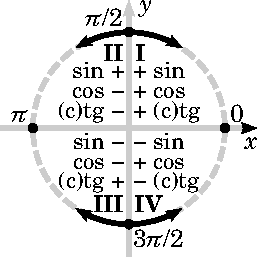
\includegraphics{drawing.pdf}\par}
\end{column*}

{\bold Следствие.} Для обратных функций верно:\par
% ---
\begin{tabularc}{0pt}{0pt}{c @{\quad\quad} c}{c}
\parbox{136pt}{\begin{align*}
\arcsin x+\arccos x&=\pi/2\\
\arctg x+\arcctg x&=\pi/2
\end{align*}} &
\parbox{143pt}{\begin{align*}
\arccos x+\arccos(-x)&=\pi\\
\arcctg x+\arcctg(-x)&=\pi
\end{align*}}
\end{tabularc}

\vspace*{-6pt}
\subsection{Формулы понижения степени}

Из формул двойного угла и основного тригонометрического тождества следует:\par
% ---
\begin{tabularc}{0pt}{0pt}{c @{\quad\quad} c}{c}
\parbox{102pt}{\begin{align*}
\cos^2\frac{\alpha}{2}&=\frac{\cos\alpha+1}{2}\\
\sin\trsp^2\frac{\alpha}{2}&=\frac{1-\cos\alpha}{2}
\end{align*}} &

\parbox{102pt}{\begin{align*}
\tg\trsp^2\frac{\alpha}{2}&=\frac{1-\cos\alpha}{\cos\alpha+1}\\
\ctg\trsp^2\frac{\alpha}{2}&=\frac{1-\cos\alpha}{\cos\alpha+1}
\end{align*}}
\end{tabularc}

Из них легко выводятся формулы {\ital половинного угла}.

\subsection{Сумма и разность двух функций}

Из формул суммы и разности двух углов следует:
% ---
\begin{align*}
\sin\alpha\pm\sin\beta&=2\sin\frac{\alpha\pm\beta}{2}\cos\frac{\alpha\mp\beta}{2}\\[-2pt]
\cos\alpha+\cos\beta&=2\cos\frac{\alpha+\beta}{2}\cos\frac{\alpha-\beta}{2}\\[-2pt]
\cos\alpha-\cos\beta&=-2\sin\frac{\alpha+\beta}{2}\sin\frac{\alpha-\beta}{2}\\
\end{align*}\\[-34pt]
% ---
$$a\sin\alpha+b\cos\alpha=c\sin(\alpha+\phi)=c\cos(\alpha-\phi),\ c=\sqrt{a^2+b^2}$$
% ---
Из них можно вывести формулы {\ital произведения двух функций}.

{\bold Доказательство.} Рассмотрим сумму синусов:
% ---
$$\sin(x+y)+\sin(x-y)=$$
$$\sin x\cos y+\sin y\cos x+\sin x\cos y-\sin y\cos x=2\sin x\cos y$$
% ---
Введём обозначения:
% ---
$$\begin{cases}
x+y=\alpha\\
x-y=\beta
\end{cases}\hspace*{-12pt}\iff
\begin{cases}
2x=\alpha+\beta\\
2y=\alpha-\beta
\end{cases}\hspace*{-12pt}\iff
\begin{cases}
x=\frac{\alpha+\beta}{2}\\
y=\frac{\alpha-\beta}{2}
\end{cases}$$
% ---
Таким образом,
% ---
$$\sin\alpha+\sin\beta=2\sin\frac{\alpha+\beta}{2}\cos\frac{\alpha-\beta}{2}.\qedw$$
% ---
Похожие формулы доказываются аналогично.$\qedw$\par

Рассмотрим синус суммы двух углов:
% ---
$$c\sin(\alpha+\phi)=c\sin\alpha\cos\phi+c\sin\phi\cos\alpha$$
% ---
Обозначим $a=c\cos\phi$, $b=c\sin\phi$ и найдём сумму квадратов:
% ---
$$a^2+b^2=c^2(\sin\trsp^2\phi+\cos^2\phi)=c^2\iff c=\sqrt{(a^2+b^2)}\qedw$$
% ---
Случай с косинусом доказывается аналогично.$\qedb$

\subsection{Подстановка Вейерштрасса}

Тригонометрические функции от $\alpha$ можно выразить через тангенс от $\alpha/2$
{\ital\color{desc}(К. Вейерштрасс)}:
% ---
$$\sin\alpha=\frac{2\tg\frac{\alpha}{2}}{1+\tg\trsp^2\frac{\alpha}{2}}\quad\quad
\cos\alpha=\frac{1-\tg\trsp^2\frac{\alpha}{2}}{1+\tg\trsp^2\frac{\alpha}{2}}$$
% ---
{\bold Доказательство.} Распишем каждую функцию:
% ---
$$\sin\alpha=\frac{2\sin\frac{\alpha}{2}\cos\frac{\alpha}{2}}{\sin\trsp^2\frac{\alpha}{2}
+\cos^2\frac{\alpha}{2}}=\frac{2\tg\frac{\alpha}{2}}{1+\tg\trsp^2\frac{\alpha}{2}}\qedw$$
$$\cos\alpha=\frac{\cos^2\frac{\alpha}{2}-\sin\trsp^2\frac{\alpha}{2}}{\sin\trsp^2\frac
{\alpha}{2}+\cos^2\frac{\alpha}{2}}=\frac{1-\tg\trsp^2\frac{\alpha}{2}}{1+\tg\trsp^2\frac
{\alpha}{2}}\qedb$$

\section{Теория множеств}

\subsection{Открытое множество}

{\ital $\varepsilon$-окрестность} точки $x_0\in X$ метрического пространства
$\langle X,d\rangle$ --- такое множество точек $x\in X$, что $d(x_0,x)\less\varepsilon$.

Упрощённая запись $\{x\mid d(x_0,x)\less\varepsilon\}=:U_\varepsilon(x_0)$.

Особые случаи:
% ---
\begin{align*}
U_\varepsilon(+\infty)&:=(1/\varepsilon;+\infty)\\
U_\varepsilon(-\infty)&:=(-\infty;-1/\varepsilon)
\end{align*}
% ---
{\ital Проколотой} называется $\varepsilon$-окрестность точки $x_0$ без неё:\\[-8pt]
% ---
$$\overset{\circ}{U}_\varepsilon(x_0):=U_\varepsilon(x_0)\backslash\{x_0\}$$
% ---
{\ital Правосторонней (левосторонней)} называется $\varepsilon$-окрестность точки $x_0$
без левой (правой) половины:
% ---
$$U_{\varepsilon+}(x_0):=[x_0;\varepsilon)\quad\quad U_{\varepsilon-}(x_0):=(\varepsilon;x_0]$$

\subsection{Ограниченное множество}

Множество $M$ ограничено {\ital сверху}, если
% ---
$$\forall m\in M\ \exists C\in\mathbb{R}\colon m\leq C.$$
% ---
{\bold Точной} {\ital (минимальной}, англ. {\ital supremum)} называется такая
{\ital верхняя} граница множества $M$ --- $\sup M$, что
% ---
$$\forall\varepsilon\greater 0\ \exists m\in M\colon m\in U_{\varepsilon-}(\sup M).$$
% ---
Множество $M$ ограничено {\ital снизу}, если
% ---
$$\forall m\in M\ \exists C\in\mathbb{R}\colon m\geq C.$$
% ---
{\bold Точной} {\ital (максимальной}, англ. {\ital infimum)} называется такая
{\ital нижняя} граница множества $M$ --- $\inf M$, что
% ---
$$\forall\varepsilon\greater 0\ \exists m\in M\colon m\in U_{\varepsilon+}(\inf M).$$

\subsection{Принцип Кантора}

Последовательность вложенных отрезков содержит точки $\xi$, которые принадлежат им всем:
% ---
$$\forall n\in\mathbb{N}\ \exists\xi\in[a_n;b_n]\subset[a_{n-1};b_{n-1}]$$
% ---
Если $n\to\infty$, $(b_n-a_n)\to 0$, то $\xi$ единственна:
% ---
$$\lim_{n\to\infty}a_n=\sup\{a_n\}=\lim_{n\to\infty}b_n=\inf\{b_n\}=\xi$$
% ---
{\bold Доказательство.} По теореме Вейерштрасса:
% ---
$$\lim_{n\to\infty}a_n=\sup\{a_n\}\quad\quad\lim_{n\to\infty}b_n=\inf\{b_n\}$$
% ---
Значит, $\forall(n\in\mathbb{N},\ \xi\in[\sup\{a_n\};\inf\{b_n\}])\ \xi\in[a_n;b_n]$.
$\qedw$

Если $\inf\{b_n\}=\sup\{a_n\}$, то $\xi$ единственна:
% ---
$$0=\inf\{b_n\}-\sup\{a_n\}=\lim_{n\to\infty}b_n-\lim_{n\to\infty}a_n=\lim_{n\to\infty}
(b_n-a_n)\qedb$$

\subsection{Локальный экстремум}

{\ital Локальный} {\bold максимум} функции $f$ --- такая точка $x_0$, что
% ---
$$\exists\delta\greater 0\colon\sup U_\delta(x_0)=f(x_0).$$ 
% ---
{\ital Локальный} {\bold минимум} функции $f$ --- такая точка $x_0$, что
% ---
$$\exists\delta\greater 0\colon\inf U_\delta(x_0)=f(x_0).$$
% ---
 Их объединяют в точки {\ital локального} {\bold экстремума}.
 
{\ital Критической} называется такая точка $x_0$, что
% ---
$$\begin{sqcases}
f'(x_0)=0\text{ \ital\color{desc}(стационарна)}\\
f'(x_0)=\text{undefined}
\end{sqcases}$$

\section{Алгебра логики}

\subsection{Определение}

{\bold Алгебра логики} --- алгебраическая структура, которая образована двухэлементным множеством $\{0;1\}$.

{\bold Высказывание} --- повествовательное предложение, о кото"=ром можно сказать в данный момент, что оно {\ital истинно} или {\ital ложно}.

{\bold Логическая связка} --- операция алгебры логики:
% ---
\begin{list*}[][\#]
\item{\ital Инверсия} «$\lnot$» --- логическое {\ital «не»}.
\item{\ital Конъюнкция} «$\land$» --- логическое {\ital «и»}.
\item{\ital Дизъюнкция} «$\lor$» --- логическое {\ital «или»}.
\item{\ital Строгая дизъюнкция} «$\dot{\lor}$» --- логическое {\ital «искл. или»}.
\item{\ital Импликация} «$\rightarrow$» --- логическое {\ital «$\implies$»}.
\item{\ital Эквиваленция} «$\equiv$» --- логическое {\ital «$\iff$»}.
\end{list*}

\subsection{Свойства}

Конъюнкция и дизъюнкция {\ital коммутативны}, {\ital ассоциативны} и {\ital дистрибутивны} относительно друг друга.
% ---
\begin{theorem}
{\bold Идемпотентность.}
% ---
$$A\land A=A\qquad A\lor A=A$$
\end{theorem}
% ---
\begin{theorem}
{\bold Закон противоречия} и {\bold исключённого третьего.}
% ---
$$A\land\overline{A}=0\qquad A\lor\overline{A}=1$$
\end{theorem}
% ---
\begin{theorem}
{\bold Закон поглощения.}
% ---
$$\begin{aligned}
&A\land 1=A &\quad &A\land 0=0\\
&A\lor 1=1 &\quad &A\lor 0=A
\end{aligned}$$
\end{theorem}
% ---
\begin{theorem}
{\bold Закон де Мóргана.}
% ---
$$\overline{A\land B}=\overline{A}\lor\overline{B}\qquad\overline{A\lor B}=\overline{A}\land\overline{B}$$
\end{theorem}

\subsection{Нормальная форма}

{\bold Терм} --- компонент логической функции:

\begin{list*}
\item{\bold макстерм} --- переменные прямой и инверсной форм связаны {\ital дизъюнкцией};
\item{\bold минтерм} --- переменные прямой и инверсной форм связаны {\ital конъюнкцией};
\end{list*}

{\bold Ранг} {\ital терма} --- число переменных, которые в него входят.

{\bold Нормальная дизъюнктивная форма} {\ital (DNF)} --- дизъюнк"=ция минтермов любого ранга.

{\bold Нормальная конъюнктивная форма} {\ital (CNF)} --- конъюнк"=ция макстермов любого ранга:
% ---
\begin{theorem}
\begin{tabularcx}{0pt}{0pt}{C@{\hspace*{-16pt}}C}{\textwidth}
$\begin{aligned}
A\dot{\lor}B&=(A\lor B)\land(\overline{A}\lor\overline{B})\\
A\equiv B&=(\overline{A}\lor B)\land(A\lor\overline{B})
\end{aligned}$\hspace*{-18pt} & $A\rightarrow B=\overline{A}\lor B$
\end{tabularcx}
\end{theorem}
% ---
{\bold Нормальная импликативная форма} {\ital (INF)} --- конъюнк"=ция макстермов любого ранга, которые заменены имплика"=цией:
% ---
$$A\lor B=(\overline{A}\rightarrow B)\land(\overline{B}\to A)$$

\section{Общая алгебра}

\subsection{Соответствие}

{\bold Соответствие} {\ital (бинарное отношение)} между множествами
$X$~и $Y$ --- произвольное множество $\rho\subseteq X\times Y$.\par
% ---
Упрощённая запись $x\in X,\ y\in Y$, $\langle x, y\rangle\in\rho=:x\rho y$.\par

\begin{tabularc}{0pt}{0pt}{r @{ --- } l}{n}
$X\supseteq D_\rho$ & область определения {\ital (прообраз)} соответствия;\\
$Y\supseteq E_\rho$ & область значений {\ital (образ)} соответствия.
\end{tabularc} 

Соответствие $\rho$ {\ital инъективно}, когда
% ---
$$\forall x_1,x_2\in D_\rho\ \exists y\in E_\rho\colon x_1\rho y,\ x_2\rho y\iff
x_1=x_2.$$
% ---
Соответствие $\rho$ {\ital функционально}, когда
% ---
$$\forall x\in D_\rho\ \exists! y\in E_\rho\colon x\rho y.$$
% ---
Такое соответствие называется {\bold отображением} {\ital (функцией)}
и обозначается:
% ---
$$\rho\colon X\xrightarrow{x\mapsto y} Y$$
% ---
Соответствие $\rho$ {\ital сюръективно}, когда
% ---
$$\forall y\in Y\ \exists x\in D_\rho\colon x\mapsto y.$$
% ---
Соответствие $\rho$ {\ital всюду определено}, когда
% ---
$$\forall x\in X\ \exists y\in E_\rho\colon x\mapsto y.$$

\subsection{Свойства соответствий}

Пусть $\ast\subseteq X\times X$, $\circ\subseteq X\times X$ --- произвольные
соответствия.\par

Соответствие $\ast$ {\ital ассоциативно}, когда
% ---
$$\forall x,y,z\in X\implies (x\ast y)\ast z=x\ast (y\ast z).$$
% ---
Соответствие $\ast$ {\ital коммутативно}, когда
% ---
$$\forall x,y\in X\implies x\ast y=y\ast x.$$
% ---
Соответствие $\ast$ {\ital дистрибутивно} относительно $\circ$, когда
% ---
$$\forall x,y,z\in X\implies
\begin{cases}
x\ast(y\circ z)=x\ast y\circ x\ast z\\
(y\circ z)\ast x=y\ast x\circ z\ast x
\end{cases}\hspace{-12pt}.$$

\subsection{Композиция отображений}

Для отображений $f\colon X\to Y,\ g\colon Y\to Z$ существует $h\colon X\to Z$,
которое называется их {\bold композицией}.\par

Упрощённая запись $\forall x\in X\ h(x)=g(f(x))=(g\circ f)(x)$.

Композиция {\ital ассоциативна}, однако {\ital не коммутативна}.

\subsection{Ограничение и продолжение}

{\ital Ограничением} отображения $f\colon X\to Y$ на $S\subseteq D_f$ называется
такое $f\vert_S\colon S\to Y$, что
% ---
$$\forall s\in S\colon f\vert_S(s)=f(s).$$
% ---
В свою очередь, $f$ является {\ital продолжением} отображения $f\vert_S$.\par

\subsection{Метрическое пространство}

{\ital Метрическое пространство} --- алгебраическая структура $\langle M;\ d\rangle$,
где $d$ --- метрика.\par

Метрика $d$ множества $M$ --- функция $d\colon M\times M\to R^+_0$, которая
определяет {\ital расстояние} между его двумя элементами.\par

Например, {\ital евклидова метрика} использует теорему Пифагора в $n$-мерном
пространстве:
% ---
$$d(x,y)=\sqrt{\sum^{n}_{k=1}(x_k-y_k)^2}$$
% ---
Для метрического пространства $\langle M;\ d\rangle,\ x,y,z\in M$ выполня"=ются
следующие {\ital аксиомы}:\par

--- $d(x,y)=0\iff x=y$ --- {\ital тождество};\\
--- $d(x,y)=d(y,x)$ --- {\ital симметрия};\\
--- $d(x,y)\leq d(x,z) + d(y,z)$ --- {\ital «неравенство треугольника»}.

\subsection{Алгебраическая операция}

Отображение $\ast\colon X^n\to X$ называется $n$-местной {\ital алгебраичес"=кой 
операцией} на $X$.\par

{\ital Нейтральным} называется такой элемент $e\in X$, что
% ---
$$\forall x\in X\implies e\ast x=x\text{ и }x\ast e=x.$$
% ---
{\bold Левым} или {\bold правым} {\ital нейтральным} называется такой элемент
$e\in X$, что
% ---
$$\forall x\in X\implies e\ast x=x\text{ или }x\ast e=x.$$
% ---
Если $x\ast y=e$, то $x$ --- {\bold левый} {\ital обратный} элемент к $y$, а $y$ ---
{\bold правый} {\ital обратный} к $x$.\par

Стоит отметить, что если $y\colon X\to Y$ и $x\colon Y\to X$ --- отображе"=ния, то $y$ 
{\ital инъективно}, а $x$ {\ital сюръективно}.\par

{\bold Доказательство.} По условию, множество $X$ накладывается на себя.
Значит, $f$ {\ital всюду определено}.\par

Так как $g$ функционально, то
% ---
$$\forall x_1,x_2\in X\ \exists y\in E_f\colon x_1fy,\ x_2fy\iff x_1=x_2,$$
% ---
то есть $f$ {\ital инъективно}.$\qedw$\par

Когда $X$ накладывается на себя, то
% ---
$$\forall x\in E_g\ \exists y\in D_g\colon x\mapsto y,$$
% ---
то есть $g$ {\ital сюръективно}.$\qedb$

Элементы $x$ и $y$ {\bold взаимно} {\ital обратны}, когда $x\ast y=y\ast x=e$.

\newpage
\subsection{Алгебраическая структура}

{\bold Алгебраическая структура} {\ital (система)} --- множество $X$ с~введёнными на нём 
алгебраическими операциями:
% ---
$$\langle X;\ \ast_1,\ast_2,\dots,\ast_n\rangle$$
% ---
{\ital Полугруппа} --- алгебраическая структура $\langle X;\ \ast\rangle$ с двухмест"=ной 
ассоциативной операцией $\ast$.

{\ital Группа} --- полугруппа, для которой существуют нейтраль"=ный и обратный элементы.
\par

{\ital Кольцо} --- коммутативная аддитивная группа, мультиплика"=тивная полугруппа, где
$\times$ дистрибутивно относительно $+$.\par

{\ital Поле} --- коммутативное кольцо с обратным элементом для $\times$.

\subsection{Числовые системы}

{\ital Система натуральных чисел} --- коммутативная аддитивная и мультипликативная полугруппа $\langle\mathbb{N};\ +,\times\rangle$.\par

{\ital Система целых чисел} --- коммутативное кольцо $\langle\mathbb{Z};\ +,\times\rangle$.
\par

{\ital Система рациональных чисел} --- упорядоченное поле $\langle\mathbb{Q};\ +,\times
\rangle$.\par

{\ital Система действительных чисел} --- непрерывное упорядо"=ченное поле $\langle\mathbb
{R};\ +,\times\rangle$.

{\ital Проективно расширенная числовая прямая} --- расширение множества действительных 
чисел $\widehat{\mathbb{R}}=\mathbb{R}\cup\{\infty\}$:
% ---
\begin{alignat*}{2}
a\pm\infty&=\infty\pm a=\infty,\quad &&a\neq\infty\\
b\cdot\infty&=\infty\cdot b=\infty, &&b\neq 0\\
\end{alignat*}\\[-26pt]
% ---
$$\frac{a}{\infty}=0\quad\quad\frac{b}{0}=\infty$$

\newpage
\subsection{Комплексные числа}

{\ital Система комплéксных чисел} --- непрерывное поле $\langle\mathbb{C};\ +,
\times\rangle$, в котором существует такая {\ital мнимая единица} $i$, что $i^2=-1$:
% ---
$$(a,b)\pm(c,d)=(a\pm c,b\pm d)$$
$$(a,b)(c,d)=(ac-bd,bc+ad)$$
$$1/z=\bar z/z\bar z=\bar z/\abs{z}\trsp^2$$\\
% ---
\begin{tabularc}{0pt}{0pt}{r @{ --- } l}{n}
$z=a+bi$ & комплексное число;\\
$\bar z=a-bi$ & комплексное число, {\ital сопряжённое} к $z$.
\end{tabularc}

Операция сопряжения {\ital дистрибутивна} относительно $+,\ \times$.

Алгебраическая форма числа $z=(a,b)\in\mathbb{C}$ --- $a+bi$:

\begin{tabularc}{0pt}{0pt}{r @{ --- } l}{n}
$a=:\ren{z}$ & действительная часть $z$;\\
$b=:\imn{z}$ & мнимая часть $z$.
\end{tabularc}
% ---
Извлечение квадратного корня из $z=a+bi$:
% ---
$$\sqrt{z}=\pm\left(\sqrt{\frac{\abs{z}+a}{2}}+\sgnb{b}i\sqrt{\frac{\abs{z}-a}{2}}\right)
$$
% ---
{\bold Доказательство.} По определению нужно найти такое $v$, что
% ---
$$v^2=(x+yi)^2=x^2+2xyi-y^2=a+bi=z.$$
% ---
Получаем систему уравнений:
% ---
$$\begin{cases}
x^2-y^2=a\\
2xy=b
\end{cases}\hspace*{-12pt}\iff
+\begin{cases}
(x^2-y^2)^2=a^2\\
4x^2y^2=b^2
\end{cases}\hspace*{-12pt}\iff
(x^2+y^2)^2=\abs{z}\trsp^2$$
% ---
Извлечём корень из обеих частей уравнения:
% ---
$$\pm\begin{cases}
x^2+y^2=\abs{z}\\
x^2-y^2=a
\end{cases}\hspace*{-12pt}\iff
\begin{cases}
2x^2=\abs{z}+a\\
2y^2=\abs{z}-a
\end{cases}\hspace*{-12pt}\iff$$
$$x=\pm\sqrt{\frac{\abs{z}+a}{2}},\quad y=\pm\sqrt{\frac{\abs{z}-a}{2}}$$
% ---
Так как $xy=b/2$, то при $b\geq 0\implies\sgnn{x}=\sgnn{y}$, иначе
$\sgnn{x}=-\sgnn{y}$. В общем виде это записывается так:
% ---
$$v=\pm\left(\sqrt{\frac{\abs{z}+a}{2}}+\sgnb{b}i\sqrt{\frac{\abs{z}-a}{2}}\right)\qedb$$
% ---
Тригонометрическая форма числа $z\in\mathbb{C}$ --- $r(\cos\phi+i\sin\phi)$, где $r$ --- 
модуль числа $z$, $\phi=:\arg z\in(-\pi;\pi]$ --- его аргумент {\ital (угол между 
вектором числа $z$ и начальным радиусом)}:
% ---
$$\phi=\begin{cases}
\arctg(\imn{z}/\ren{z}), &x\greater 0\\
\arctg(\imn{z}/\ren{z})+\pi, &x\less 0,\ y\geq 0\\
\arctg(\imn{z}/\ren{z})-\pi, &x\less 0,\ y\less 0\\
\sgnb{\imn{z}}\pi/2, &x=0,\ y\neq 0
\end{cases}$$
% ---
Произведение чисел $z_1,z_2\in\mathbb{C}$ --- число с модулем $\abs{z_1z_2}=$
$\abs{\abs{z_1}\cdot\abs{z_2}}$ и аргументом $\arg(z_1z_2)=\arg z_1+\arg z_2$.

{\bold Следствие.} Возведение в степень числа $z=r(\cos\phi+i\sin\phi)$:
% ---
$$z^n=r^n(\cos n\phi+i\sin n\phi),\ n\in\mathbb{Z}$$
% ---
Частное чисел $z_1,z_2\in\mathbb{C}$ --- число с модулем $\abs{z_1/z_2}=$
$\abs{\abs{z_1}/\abs{z_2}}$ и аргументом $\arg(z_1/z_2)=\arg z_1-\arg z_2$.

Извлечение корня $n$ степени из $z=r(\cos\phi+i\sin\phi)$:
% ---
$$\sqrt[n]{z}=\sqrt[n]{r}\left(\cos\frac{\phi+2\pi k}{n}+i\sin\frac{\phi+2\pi k}{n}
\right),\ k\in\{m\}_{m=0}^{n-1}$$
% ---
{\bold Доказательство.} По определению нужно найти такое $v$, что
% ---
$$v^n=\rho^n(\cos n\alpha+i\sin n\alpha)=r(\cos\phi+i\sin\phi)=z$$
% ---
Получаем систему уравнений:
% ---
$$\begin{cases}
\rho^n=r\\
n\alpha=\phi+2\pi k
\end{cases}\hspace{-12pt}\iff\begin{cases}
\rho=\sqrt[n]{r}\\
\alpha=(\phi+2\pi k)/n,\ k\in\mathbb{Z}
\end{cases}$$
% ---
Значит,
% ---
$$v=\sqrt[n]{r}\left(\cos\frac{\phi+2\pi k}{n}+i\sin\frac{\phi+2\pi k}{n}\right).
\qedb$$

\section{Вычислительная геометрия}

\subsection{Деление отрезка в отношении}

Точка $C$ делит отрезок $AB$ в отношении $\lambda\in\mathbb{R}$, если:
% ---
$$\begin{cases}
C\in AB\\
\overrightarrow{AC}=\lambda\overrightarrow{CB}\\
\lambda\neq -1
\end{cases}$$
% ---
\begin{theorem}
{\bold Теорема.} Пусть $C$ делит $AB$ в отношении $\lambda\in\mathbb{R}$. Тогда координаты точки $C$ равны:
% ---
$$x_C=\frac{x_A+\lambda x_B}{1+\lambda}\qquad y_C=\frac{y_A+\lambda y_B}{1+\lambda}$$ 
\end{theorem}

{\bold Доказательство.} По условию:
% ---
$$\overrightarrow{AC}=\lambda\overrightarrow{CB}\iff\overrightarrow{OC}-\overrightarrow{OA}=\lambda(\overrightarrow{OB}-\overrightarrow{OC})$$
% ---
По теореме Фалеса:
% ---
$$\left\{\begin{aligned}
&x_C-x_A=\lambda(x_B-x_C)\\
&y_C-y_A=\lambda(y_B-y_C)
\end{aligned}\right.\iff
\left\{\begin{aligned}
&x_C=\frac{x_A+\lambda x_B}{1+\lambda}\\
&y_C=\frac{y_A+\lambda y_B}{1+\lambda}
\end{aligned}\right.\qedb$$

\subsection{Коллинеарность}

{\bold Коллинеарными} называются:
% ---
\begin{tabularcx}{3pt}{3pt}{@{--- } L}{\textwidth}
{\ital точки}, которые лежат на одной прямой;\\
{\ital векторы}, которые лежат на одной прямой или на~параллельных прямых.
\end{tabularcx}
% ---
\begin{theorem}
{\bold Критерий коллинеарности} двух векторов:
% ---
$$\overrightarrow{a}=\lambda\overrightarrow{b},\ \lambda\in\mathbb{R}\iff\begin{cases}
x_a=\lambda x_b\\
y_a=\lambda y_b
\end{cases}$$ 
\end{theorem}
% ---
В частности, нулевой вектор коллинеарен {\ital любому} вектору:
% ---
$$\overrightarrow{0}=0\overrightarrow{a}$$
% ---
\begin{theorem}
{\bold Уравнение секущей} по двум известным точкам:
% ---
$$A\langle x_a,y_a\rangle,\ B\langle x_b,y_b\rangle\implies\frac{x-x_a}{x_b-x_a}=\frac{y-y_a}{y_b-y_a}$$
\end{theorem}
% ---
{\bold Доказательство.} Пусть $\overrightarrow{AX},\ \overrightarrow{AB}$ --- коллинеарные векторы.

По критерию коллинеарности двух векторов:
% ---
$$\left\{\begin{aligned}
x-x_a=\lambda(x_b-x_a)\\
y-y_a=\lambda(y_b-y_a)
\end{aligned}\right.\iff
\lambda=\frac{x-x_a}{x_b-x_a}=\frac{y-y_a}{y_b-y_a}\qedb$$

\subsection{Скалярное произведение}

\begin{theorem}
{\bold Теорема.} Косинус угла $\alpha$ между векторами $\overrightarrow{a}$ и $\overrightarrow{b}$ равен:
% ---
$$\cos\alpha=\frac{x_ax_b+y_ay_b}{\abs{\overrightarrow{a}}\abs{\overrightarrow{b}}}$$
\end{theorem}
% ---
{\bold Доказательство.} Отложим векторы $\overrightarrow{AB}=\overrightarrow{a}$, $\overrightarrow{AC}=\overrightarrow{b}$ от начала координат.

По теореме косинусов:
% ---
$$\begin{gathered}
BC^2=AB^2+AC^2-2\abs{\overrightarrow{AB}}\abs{\overrightarrow{AC}}\cos\alpha\implies\\
\cos\alpha=\frac{AB^2+AC^2-BC^2}{2\abs{\overrightarrow{AB}}\abs{\overrightarrow{AC}}}
\end{gathered}$$
% ---
По теореме Пифагора:
% ---
$$\begin{gathered}
\left\{\begin{aligned}
&AB^2=x_a^2+y_a^2\\
&AC^2=x_b^2+y_b^2\\
&BC^2=(x_a-x_b)^2+(y_a-y_b)^2
\end{aligned}\right.\implies\\
AB^2+AC^2-BC^2=2(x_ax_b+y_ay_b)\implies\\
\cos\alpha=\frac{x_ax_b+y_ay_b}{\abs{\overrightarrow{a}}\abs{\overrightarrow{b}}}\qedb
\end{gathered}$$
% ---
{\bold Скалярное произведение} {\ital векторов} $\overrightarrow{a}$, $\overrightarrow{b}$ --- величина:
% ---
$$x_ax_b+y_ay_b=:\overrightarrow{a}\cdot\overrightarrow{b}$$
% ---
\begin{theorem}
{\bold Теорема.} Скалярное произведение двух векторов равно:
% ---
$$\overrightarrow{a}\cdot\overrightarrow{b}=\abs{\overrightarrow{a}}\abs{\overrightarrow{b}}\cos\alpha,$$
% ---
$\alpha$ --- угол между векторами.
\end{theorem}

\begin{theorem}
{\bold Теорема.} Если вектора $\overrightarrow{a}$ и $\overrightarrow{b}$ коллинеарны, то:

\begin{list*}
\item$\overrightarrow{a}\cdot\overrightarrow{b}\greater 0\implies$ вектора {\ital сонаправлены};
\item$\overrightarrow{a}\cdot\overrightarrow{b}\less 0\implies$ вектора {\ital несонаправлены};
\item$\overrightarrow{a}\cdot\overrightarrow{b}=0\implies$ один из векторов {\ital нулевой}.
\end{list*}
\end{theorem}

\subsection{Ориентированный угол}

{\bold Ориентированным} называется угол $\alpha$ между $\overrightarrow{a}$ и $\overrightarrow{b}$, на который нужно повернуть $\overrightarrow{a}$, чтобы он был сонаправлен с $\overrightarrow{b}$:
% ---
$$\angle(\overrightarrow{a},\overrightarrow{b})\text{ --- обозначение},\ \alpha\in\left(-\pi;\pi\right]$$
% ---
{\bold Знак} ориентированного угла:

\begin{list*}
\item{\bold пололжительный}, если поворот происходит в {\ital положи"=тельном} направлении системы координат;
\item{\bold отрицательный}, если поворот происходит в {\ital отрица"=тельном} направлении системы координат;
\item{\bold нуль}, если вектора {\ital сонаправлены}.
\end{list*}

\subsection{Косое произведение}

{\bold Косое произведение} {\ital векторов} $\overrightarrow{a}$, $\overrightarrow{b}$ --- величина:
% ---
$$x_ax_b-y_ay_b=:\overrightarrow{a}\land\overrightarrow{b}$$
% ---
\begin{theorem}
{\bold Теорема.} Косое произведение двух векторов равно:
% ---
$$\overrightarrow{a}\land\overrightarrow{b}=\abs{\overrightarrow{a}}\abs{\overrightarrow{b}}\sin\alpha,$$
% ---
$\alpha$ --- угол между векторами.
\end{theorem}

\begin{theorem}
{\bold Теорема.} Знак косого произведения векторов {\ital совпадает} со знаком ориентированного угла.
\end{theorem}

Доказательство вытекает из {\ital чётности} синуса угла между векторами.

\subsection{Взаимное расположение объектов}

Расположение {\ital точки} $A$ относительно {\ital прямой, луча или отрезка} $BC$:

\begin{list*}
\item$\angle(\overrightarrow{BA},\overrightarrow{BC})\greater 0\implies A$ лежит в {\bold левой} полуплоскости;
\item$\angle(\overrightarrow{BA},\overrightarrow{BC})\less 0\implies A$ лежит в {\bold правой} полуплоскости;
\item$\angle(\overrightarrow{BA},\overrightarrow{BC})=0\implies A$ {\bold коллинеарна} прямой $BC$.
\end{list*}

Взаимное расположение {\ital двух отрезков или лучей} $AB$ и $CD$:

\begin{list*}
\item концы обоих отрезков лежат в {\ital разных} полуплоскостях относительно друг друга $\implies$ отрезки {\bold пересекаются};
\item концы одного отрезка лежат в {\ital одной} полуплоскости относительно другого $\implies$ отрезки {\bold не пересекаются};
\item концы одного отрезка лежат {\ital на} прямой другого отрезка:
\begin{list*}[2]
\item конец одного отрезка лежит {\ital на} другом $\implies$ отрезки имеют {\bold общий подотрезок};
\item концы одного отрезка {\ital не} лежат на другом $\implies$ отрезки {\bold не пересекаются}.
\end{list*}
\end{list*}

\subsection{Ориентированная площадь}

{\bold Ориентированной} называется площадь многоугольника, которая обладает знаком его ориентированных углов.

\begin{theorem}
{\bold Теорема.} Ориентированная площадь треугольника равна половине {\ital косого произведения} векторов ориентированного угла.
\end{theorem}

Ориентированная площадь --- {\ital аддитивная} величина, к~основным методам её расчёта относят:

\begin{list*}
\item метод трапеций;
\item метод треугольников.
\end{list*}

\subsection{Метод трассировки луча}

\begin{theorem}
{\bold Задача.} На плоскости даны многоугольник и точка. Решить вопрос о принадлежности точки многоугольнику.
\end{theorem}

{\bold Алгоритм} трассировки луча:

\begin{list*}[][\#]
\item Проверить принадлежность точки стороне многоуголь"=ника: если {\ital истина}, остановить алгоритм.
\item Выпустить из точки в случайном направлении луч.
\item Посчитать число $n$ пересечений луча со сторонами многоугольника:
% ---
$$\left\{\begin{aligned}
&n\equiv 0\modb{2}\implies\text{ точка снаружи}\\
&n\equiv 1\modb{2}\implies\text{ точка внутри}
\end{aligned}\right.$$
\end{list*}

\subsection{Метод заметающей прямой}

Да.

\section{Предел последовательности}

% ОПРЕДЕЛЕНИЕ ПОДПОСЛЕДОВАТЕЛЬНОСТИ

\subsection{Определение}

{\bold Предел} последовательности $\{x_n\}$ --- такое $a$, что
% ---
$$\forall\varepsilon\greater 0\ \exists N\colon\forall n\greater N\ x_n\in U_
\varepsilon(a).$$
% ---
Упрощённая запись $\lim_{n\to\infty}x_n=a$ или $n\to\infty$, $x_n\to a$.

Этот оператор {\ital «дистрибутивен»} относительно {\ital сложения}, {\ital умножения} и {\ital деления {\color{desc}(предел знаменателя не равен нулю)}}.

{\bold Частичным} называется предел подпоследовательности.

\subsection{Свойства}

\begin{theorem}
Сходимость $\implies$ ограниченность.
\end{theorem}
% ---
{\bold Доказательство.} Пусть $\lim_{n\to\infty}x_n=a$. По определению:
% ---
$$\forall\varepsilon\greater 0\ \exists N\colon\forall n\greater N\ x_n\in U_
\varepsilon(a)$$
% ---
По «дистрибуции» модуля относительно сложения:
% ---
$$\abs{x_n}=\abs{x_n-a+a}\leq\abs{x_n-a}+\abs{a}\less\varepsilon+\abs{a}$$
% ---
Положим, что $\forall m\leq N\ L=\max(\abs{\{x_m\}},\varepsilon+\abs{a})\implies\abs{x_n}
\leq L$.$\qedb$

\begin{theorem}
{\bold Предельный переход.} Пусть $n\to\infty$, $x_n\to a$, $y_n\to b$. Тогда справедливо следствие:
% ---
$$x_n\leq y_n\text{ или }x_n\less y_n\implies a\leq b$$
\end{theorem}

{\bold Доказательство.} По определению предела:
% ---
$$\forall\varepsilon\greater 0\ \exists N\colon\forall n\greater N\ x_n\in U_
\varepsilon(a),\ y_n\in U_\varepsilon(b)$$
% ---
Следовательно,
% ---
$$+\begin{cases}
x_n\leq y_n\\
a-x_n\less\varepsilon\\
y_n-b\less\varepsilon
\end{cases}\hspace*{-12pt}\iff
\begin{cases}
y_n-x_n\geq 0\\
y_n-x_n\less 2\varepsilon+b-a
\end{cases}\hspace*{-12pt}\iff
\frac{a-b}{2}\less\varepsilon$$
% ---
Так как $\varepsilon$ --- сколь угодно малое положительное число, то $a-b\leq 0\iff a\leq 
b$.$\qedw$

При $x_n\less y_n$ доказательство аналогично.$\qedb$

\begin{theorem}
{\bold Теорема о промежуточной функции.} Пусть $n\to\infty$, $x_n,y_n\to a$. Тогда справедливо следствие:
% ---
$$\forall\{z_n\}\colon x_n\leq z_n\leq y_n\implies z_n\to a$$
\end{theorem}

{\bold Доказательство.} По определению предела:
% ---
$$\forall\varepsilon\greater 0\ \exists N\colon\forall n\greater N\ x_n,y_n\in U_
\varepsilon(a)$$
% ---
Следовательно,
% ---
$$a-\varepsilon\less x_n\leq z_n\leq y_n\less a+\varepsilon\implies z_n\in U_
\varepsilon(a)\implies\lim_{n\to\infty}z_n=a.\qedb$$

\subsection{Условие Коши}

Последовательность $\{x_n\}$ удовлетворяет {\bold условию Коши} {\ital\color{desc} 
(является фундаментальной)}, если
% ---
$$\forall\varepsilon\greater 0\ \exists N\colon\forall n,m\greater N\ \abs{x_n-x_m}\less
\varepsilon.$$
% ---
\begin{theorem}
Фундаментальность $\implies$ ограниченность.
\end{theorem}
% ---
{\bold Доказательство.} По условию Коши:
% ---
$$\forall\varepsilon\greater 0\ \exists N\colon\forall n,m\greater N\ \abs{x_n-x_m}\less
\varepsilon$$
% ---
По «дистрибуции» модуля относительно сложения:
% ---
$$\begin{cases}
\abs{x_n-x_m}\less\varepsilon\\
\abs{x_n}=\abs{x_n-x_m+x_m}
\end{cases}\hspace*{-12pt}\iff
\begin{cases}
\abs{x_n-x_m}\less\varepsilon\\
\abs{x_n}\leq\abs{x_n-x_m}+\abs{x_m}
\end{cases}\hspace*{-12pt}\iff$$
$$\abs{x_n}\less\varepsilon+\abs{x_m}$$
% ---
Положим, что $\forall k\leq N\ L=\max(\abs{\{x_k\}},\varepsilon+\abs{x_m})\implies
\abs{x_n}\leq L$.$\qedb$

\subsection{Принцип компактности отрезка}

\begin{theorem}
Ограниченность $\implies$ частичная сходимость:
% ---
$$\forall\{x_n\}\in[a;b]\ \exists\{n_k\}\kern-4pt\uparrow\colon\lim_{k\to\infty}x_{n_k}=
\xi$$
\end{theorem}
% ---
{\bold Доказательство.} По принципу Кантора:
% ---
$$\forall k\in\mathbb{N}\ \exists!\xi\in[a_k;b_k]\subset[a_{k-1};b_{k-1}]\iff$$
$$\lim_{k\to\infty}a_k=\lim_{k\to\infty}b_n=\xi$$
% ---
Образуем подпоследовательность:
% ---
$$\{x_{n_k}\mid \{n_k\}\kern-4pt\uparrow,\ x_{n_k}\in[a_k;b_k]\}$$
% ---
По теореме о промежуточной функции:
% ---
$$a_k\leq x_{n_k}\leq b_k\implies \lim_{k\to\infty}x_{n_k}=\xi\qedb$$
% ---
\begin{theorem}
Частичный предел фундаментальной последовательности является её пределом.
\end{theorem}
% ---
{\bold Доказательство.} Пусть $\{x_n\}$ фундаментальна $\implies$ она ограничена.

По принципу компактности отрезка $\lim_{k\to\infty}x_{n_k}=a$.

По условию Коши:
% ---
$$\forall\varepsilon/2\greater 0\ \exists N\colon\forall n,m\greater N\ \abs{x_n-x_m}
\less\varepsilon/2$$
% ---
Зафиксируем $n$. При $x_m=x_{n_k}\greater N$ перейдём к пределу:
% ---
$$\abs{x_n-a}\leq\varepsilon/2\less\varepsilon\iff\lim_{k\to\infty}x_n=a\qedb$$

\subsection{Критерий Коши}

\begin{theorem}
Сходимость $\iff$ фундаментальность.
\end{theorem}
% ---
{\bold Доказательство $\implies$.} По определению предела:
% ---
$$\forall\varepsilon\greater 0\ \exists N\colon\forall n\greater N\ x_n\in U_
{\varepsilon/2}(a)$$ 
% ---
Значит, $\forall n,m\greater N\ \abs{x_n-x_m}=\abs{(x_n-a)+(a-x_m)}$.

По «дистрибуции» модуля относительно сложения:
% ---
$$\abs{x_n-x_m}\leq\abs{x_n-a}+\abs{x_m-a}\less \varepsilon/2+\varepsilon/2=\varepsilon
\qedb$$
% ---
{\bold Доказательство $\impliedby$.} Пусть $\{x_n\}$ фундаментальна $\implies$ она 
ограничена $\implies$ по принципу компактности отрезка она частично сходится к $c$
$\implies$ по условию Коши и принципу компактности отрезка она сходится к $c$.$\qedb$

\subsection{Теорема Вейерштрасса}

\begin{theorem}
Монотонность $\implies$ сходимость:
% ---
$$\begin{sqcases}
\forall\{x_n\}\kern-4pt\nearrow\lim_{n\to\infty}x_n=\sup\{x_n\}\\
\forall\{y_n\}\kern-4pt\searrow\lim_{n\to\infty}y_n=\inf\{y_n\}
\end{sqcases}$$
\end{theorem}
% ---
{\bold Доказательство.} По определению точной верхней границы:
% ---
$$\forall n\in\mathbb{N}\ x_n\leq\sup\{x_n\}$$
% ---
Так как последовательность неубывает, то
% ---
$$\forall\epsilon\greater 0\ \exists N\colon\forall n\greater N\ x_n\in U_\epsilon(\sup
\{x_n\})\implies$$
$$\lim_{n\to\infty}x_n=\sup\{x_n\}.\qedw$$
% ---
Для $\{y_n\}\kern-4pt\searrow$ доказательство аналогично.$\qedb$

\section{Предел функции}

\subsection{Предел}

{\bold Предел} функции $f\colon X\to Y$ в точке $x_0\in X$ {\ital по Коши} --- такое
$a\in Y$, что {\ital\color{desc} (О.Л. Коши)}
% ---
$$\forall\varepsilon\greater 0\ \exists\delta\greater 0\colon\forall x\in\underbrace{
\overset{\circ}{U}_\delta(x_0)\subseteq D_f}_{\text{\tinyt I}},\ \underbrace{f(x)\in U_\varepsilon(a)}_{\text{\tinyt II}}.$$\\
% ---
\begin{tabularc}{0pt}{0pt}{>{\raggedleft\arraybackslash}p{.03\linewidth} @{ --- } 
>{\raggedright\arraybackslash}p{.91\linewidth}}{n}
I & функция $f$ определена в какой-либо проколотой $\delta$-окрестности точки $x_0$;
\\[18pt]
II & функция $f$ имеет образ в какой-либо проколотой $\varepsilon$-окрестности точки 
$a$.  
\end{tabularc}

{\bold Предел} функции $f\colon X\to Y$ в точке $x_0\in X$ {\ital по Гейне} --- такое
$a\in Y$, что {\ital\color{desc} (Э. Гейне)}
% ---
$$\forall\{x_n\}\in D_f\colon\lim_{n\to\infty}x_n=x_0\ (x_n\neq x_0)\implies\lim_{n\to
\infty}f(x_n)=a.$$
% ---
Упрощённая запись $\forall x\in X\ \lim_{x\to x_0}f(x)=a$ или $x\to x_0$, $f(x)\to a$.

\subsection{Критерий Коши}

Сходимость $\iff$ выполнение {\ital условия Коши}:\\[-8pt]
% ---
$$\forall\varepsilon\greater 0\ \exists\delta\greater 0\colon\forall x',x''\in\overset
{\circ}{U}_\delta(x_0)\ \abs{f(x')-f(x'')}\less\varepsilon$$
% ---
{\bold Доказательство $\implies$.} По определению предела:\\[-8pt]
% ---
$$\forall\varepsilon\greater 0\ \exists\delta\greater 0\colon\overset{\circ}{U}_\delta
(x_0)\subseteq D_f,\ U_{\varepsilon/2}(a)\cap E_f\neq\emptyset$$\\[-6pt]
% ---
Пусть $x',x''\in\overset{\circ}{U}_\delta(x_0)$; по неравенству треугольника:
% ---
$$\abs{f(x')-f(x'')}\leq\abs{f(x')-a}+\abs{f(x'')-a}\less\varepsilon/2+\varepsilon/2=
\varepsilon\qedb$$
% ---
{\bold Доказательство $\impliedby$.} По условию Коши:
% ---
$$\exists\{x_n\}\in D_f\colon\lim_{n\to\infty}x_n=x_0,\ x_n\neq x_0$$
% ---
Последовательности $\{f(x_n)\}$ фундаментальны $\implies$ сходятся.

По фундаментальности и сходимости к одной точке $x_0$:
% ---
$$\lim_{x\to x_0}f(x)=a\qedb$$

\subsection{Предел композиции функций}

Пусть $f\colon X\to Y$, $g\colon Y\to Z$. Тогда:
% ---
$$\begin{cases}
\lim_{x\to x_0}f(x)=y_0\\
\lim_{x\to x_0}g(x)=z_0
\end{cases}\hspace*{-12pt}\iff\begin{cases}
\lim_{x\to x_0}(g\circ f)(x)=z_0\\
f(x)\neq y_0
\end{cases}$$
% ---
{\bold Доказательство.} Пусть $g\circ f=\varphi$; по определению предела:\\[-9pt]
% ---
$$\begin{cases}
\forall\varepsilon\greater 0\ \exists\delta\greater 0\colon\overset{\circ}{U}_\delta(y_0)
\subseteq D_g,\ U_\varepsilon(z_0)\cap E_g\neq\emptyset\\
\forall\delta\greater 0\ \exists\sigma\greater 0\colon\overset{\circ}{U}_\sigma(x_0)
\subseteq D_f,\ U_\delta(y_0)\cap E_f\neq\emptyset
\end{cases}$$\\[-6pt]
% ---
Из $\overset{\circ}{U}_\delta(y_0)\cap U_\delta(y_0)=\overset{\circ}{U}_\delta(y_0)$ 
следует:\\[-14pt]
% ---
$$\begin{cases}
\forall\varepsilon\greater 0\ \exists\sigma\greater 0\colon\overset{\circ}{U}_\sigma(x_0)
\subseteq D_f,\ U_\varepsilon(\varphi(x))\cap E_g\neq\emptyset\\
y\neq y_0\iff f(x)\neq y_0
\end{cases}\hspace*{-12pt}\iff$$
$$\lim_{x\to x_0}\varphi(x)=z_0,\ f(x)\neq y_0.\qedb$$

\subsection{Бесконечно малая функция}

Функция $g$ {\ital бесконечно мала} относительно $f$ при $x\to\ x_0$, если
% ---
$$g(x)=\varepsilon(x)f(x):=\underset{x\to\ x_0}{o(f)},\quad\quad\lim_{x\to x_0}\varepsilon
(x)=0.$$
% ---
Верно следующее утверждение:
% ---
$$\lim_{x\to\ x_0}f(x)=a\iff f(x)=a+\underset{x\to x_0}{o(x)}$$
% ---
{\bold Доказательство $\implies$.} По определению предела:
% ---
$$\forall\varepsilon\greater 0\ \exists\delta\greater 0\colon 0\less\abs{x-x_0}\less
\delta,\ \abs{f(x)-a}\less\varepsilon$$
% ---
По теореме о промежуточной функции:
% ---
$$0\leq\abs{f(x)-a}\less\varepsilon\implies\lim_{x\to x_0}(f(x)-a)=0\iff$$
$$f(x)-a=\underset{x\to x_0}{o(x)}\iff f(x)=a+\underset{x\to x_0}{o(x)}\qedb$$
% ---
{\bold Доказательство $\impliedby$.} По условию:
% ---
$$f(x)=a+o(x)\iff\abs{f(x)-a}=\abs{o(x)}$$
% ---
По определению бесконечно малой функции:
% ---
$$\forall\varepsilon\greater 0\ \exists\delta\greater 0\colon 0\less\abs{x-x_0}\less
\delta,\ \abs{o(x)}\less\varepsilon$$
% ---
По определению предела:
% ---
$$\abs{f(x)-a}\less\varepsilon\iff\lim_{x\to x_0}f(x)=a\qedb$$

\subsection{Односторонний предел}

{\bold Правосторонним} называется предел функции, который определён в терминах
правосторонних $\varepsilon$-окрестностей {\ital (неубывающих 
последовательностей)}:
% ---
$$\lim_{x\to x_0+0}f(x)=a\quad\text{или}\quad x\to x_0+0,\ f(x)\to a$$
% ---
{\bold Левосторонним} называется предел функции, который определён в терминах
левосторонних $\varepsilon$-окрестностей {\ital (невозрастающих 
последовательностей)}.
% ---
$$\lim_{x\to x_0-0}f(x)=a\quad\text{или}\quad x\to x_0-0,\ f(x)\to a$$
% ---
Сущестование предела равносильно существованию {\ital равных} односторонних пределов:
% ---
$$\lim_{x\to x_0}f(x)\iff\lim_{x\to x_0+0}f(x)=\lim_{x\to x_0-0}f(x)$$

\subsection{Непрерывность}

Пусть $\forall\varepsilon\greater 0\ U_\varepsilon(x_0)\subseteq D_f$. Тогда:

\begin{tabularc}{0pt}{0pt}{r @{ --- } l}{n}
$x-x_0=:\Delta x$ & {\ital приращение аргумента} в точке $x_0$;\\
$f(x)-f(x_0)=:\Delta f$ & {\ital приращение функции} в точке $x_0$.
\end{tabularc}

Функция $f$ {\ital непрерывна} в точке $x_0$, если
% ---
$$\lim_{x\to x_0}f(x)=f(x_0)\quad\text{или}\quad\Delta x\to 0,\ \Delta f\to 0.$$
% ---
Определения {\ital непрерывности справа} и {\ital слева} точки $x_0$ связаны
с правосторонними и левосторонними пределами.

Непрерывными в точке $x_0$ являются {\ital сумма}, {\ital произведение} и~{\ital 
композиция} непрерывных в ней функций.

\newpage
\subsection{Теорема Вейерштрасса}

Пусть $f\in C[a;b]$. Тогда в некоторых точках отрезка функция достигает своих точных 
верхней и нижней границ на $[a;b]$.

{\bold Доказательство.} Пусть $\sup f([a;b])=:M$, $\inf f([a;b])=:m$.

По определению точных верхней и нижней границ:
% ---
$$\forall x\in[a;b]\ f(x)\in[m;M]$$
% ---
По принципу компактности отрезка:
% ---
$$\lim_{n\to\infty}f(x_n)=M\quad\quad\lim_{k\to\infty}x_{n_k}=\xi$$
% ---
По определению непрерывности:
% ---
$$\lim_{k\to\infty}f(x_{n_k})=f(\xi)\implies f(\xi)=M\qedb$$

\subsection{Теорема о промежуточном значении}

Пусть $f$ непрерывна на промежутке $X\ni a,b$. Тогда:
% ---
$$\forall c\in[f(a);f(b)]\ \exists\xi\in[a;b]\colon c=f(\xi)$$
% ---
{\bold Доказательство.} По принципу Кантора:
% ---
$$\forall n\in\mathbb{N}\ \exists\xi\in[a_n;b_n]\subset[a_{n-1};b_{n-1}]\subseteq X
\implies$$
$$n\to\infty,\ a_n,b_n\to\xi$$
% ---
По определению непрерывности функции на промежутке:
% ---
$$n\to\infty,\ f(a_n),f(b_n)\to f(\xi)$$
% ---
По теореме о промежуточной функции:
% ---
$$f(a_n)\leq c\leq f(b_n)\implies c=f(\xi)\qedb$$

\section{Дифференциальное исчисление}

% ОПРЕДЕЛЕНИЕ МОНОТОННОСТИ ОКОЛО ТОЧКИ

\subsection{Производная}

Функция $f$ имеет в точке $x_0$ {\ital производную (дифференцируема в ней)}, если {\ital
\color{desc} (Ж.Л. Лагранж)}
% ---
$$\forall\epsilon\greater 0\ U_\epsilon(x_0)\cap D_f\neq\emptyset,\ \lim_{\Delta x\to 0}
\frac{\Delta f}{\Delta x}=:f'(x_0).$$
% ---
Этот оператор {\ital дистрибутивен} относительно {\ital сложения}:
% ---
\begin{align*}
(f\cdot g)'&=f'g+fg'\\
\left(\frac{f}{g}\right)'&=\frac{f'g-fg'}{g^2}\\
(f\circ g)'&=(f'\circ g)g'
\end{align*}

\subsection{Свойства производной}

Дифференцируемость $\implies$ непрерывность.

{\bold Доказательство.} По определению производной:
% ---
$$\lim_{\Delta x\to 0}\frac{\Delta f}{\Delta x}=f'(x_0)\iff \frac{\Delta f}{\Delta x}=
f'(x_0)+o(\Delta x)\iff$$
$$\Delta f=\Delta x(f'(x_0)+o(\Delta x))\implies\Delta x\to 0,\ \Delta f\to 0\qedb$$
% ---
Приращение дифференцируемой функции легко предста"=вить в виде:
% ---
$$\Delta f=f'(x_0)\Delta x+o(\Delta x)\Delta x$$
% ---
{\ital Дифференциал функции} --- линейная часть её приращения:
% ---
$$\diff y:=f'(x_0)\Delta x$$
% ---
Значит, формула производной имеет вид:
% ---
$$f'(x_0)=\frac{\diff y}{\Delta x}=\frac{\diff y}{\diff x}\quad(\Delta x=\diff x)$$

\newpage
\subsection{Производные элементарных функций}

Таблица производных элементарных функций:

\begin{align*}
C'&=0\quad\quad & (x^n)'&=nx^{n-1}\\
\sin'\alpha&=\cos\alpha & \cos'\alpha&=-\sin\alpha\\
\tg'\alpha&=\frac{1}{\cos^2\alpha} & \ctg'\alpha&=-\frac{1}{\sin\trsp^2\alpha}\\
\arcsin'x&=\frac{1}{\sqrt{1-x^2}} & \arccos'x&=-\frac{1}{\sqrt{1-x^2}}\\
\arctg'x&=\frac{1}{1+x^2} & \arcctg'x&=-\frac{1}{1+x^2}
\end{align*}

\subsection{Промежутки монотонности}

Если функция $f$ дифференцируема в точке $x_0$, то
% ---
$$\begin{cases}
f'(x_0)\greater 0\implies f\kern-4pt\uparrow\text{около }x_0\\
f'(x_0)\less 0\implies f\kern-4pt\downarrow\text{около }x_0
\end{cases}\hspace*{-12pt}.$$

{\bold Доказательство.} По определению производной:
% ---
$$f'(x_0)\greater 0\iff \lim_{\Delta x\to 0}\frac{\Delta f}{\Delta x}\greater 0\iff\frac
{\Delta f}{\Delta x}\greater o(\Delta x)$$
% ---
При достаточно малом $\Delta x$ верно:
% ---
$$\frac{\Delta f}{\Delta x}\greater 0\iff\begin{sqcases}
\Delta f,\Delta x\greater 0\\
\Delta f,\Delta x\less 0
\end{sqcases}\hspace*{-12pt}\iff
f\kern-4pt\uparrow\text{около }x_0\qedw$$
% ---
Для $f'(x_0)\less 0$ доказательство аналогично.$\qedb$

\subsection{Условие существования экстремума}

Точка локального экстремума $\implies$ критическая точка.

{\bold Доказательство.} По определению локального максимума:
% ---
$$\exists\delta\greater 0\colon\forall x\in\overset{\circ}{U}_\delta(x_0)\ f(x_0)\greater 
f(x)$$
% ---
Производная в точке $x_0$ либо существует, либо нет.$\qedw$

Допустим, она существует; по определению производной:
% ---
$$\lim_{x\to x_0}\frac{\Delta f}{\Delta x}=f'(x_0)$$
% ---
По предельному переходу:
% ---
$$\begin{sqcases}
\Delta x\greater 0\implies\Delta f/\Delta x\less 0\implies f'(x_0)\leq 0\\
\Delta x\less 0\implies\Delta f/\Delta x\greater 0\implies f'(x_0)\geq 0
\end{sqcases}\hspace*{-12pt}\iff$$
$$0\leq f'(x_0)\leq 0\iff f'(x_0)=0\qedw$$
% ---
Для локального минимума доказательство аналогично.$\qedb$

Если в критической точке производная меняет знак, она является локальным экстремумом.

{\bold Доказательство.} По определению критической точки:
% ---
$$\begin{sqcases}
f'(x_0)=0\\
f'(x_0)=\text{undefined}
\end{sqcases}$$
% ---
Допустим для определённости:
% ---
$$\begin{cases}
\exists\delta\greater 0\colon\forall x\in\overset{\circ}{U}_{\delta-}(x_0)\ f'(x)\greater 
0\\
\exists\delta\greater 0\colon\forall x\in\overset{\circ}{U}_{\delta+}(x_0)\ f'(x)\less 0
\end{cases}$$
% ---
По промежуткам монотонности:
% ---
$$\begin{cases}
f\kern-4pt\uparrow\text{на }U_{\delta-}(x_0)\\
f\kern-4pt\downarrow\text{на }U_{\delta+}(x_0)
\end{cases}\hspace*{-12pt}\iff x_0\text{ --- локальный максимум}\qedw$$
% ---
Для локального минимума доказательство аналогично.$\qedb$

\subsection{Теорема Ролля}

Пусть $f$ дифференцируема на $(a;b)$, непрерывна на $f[a;b]$, и~$f(a)=f(b)$. Тогда: {\ital
\color{desc} (М. Ролль)}
% ---
$$\exists\xi\in(a;b)\colon f'(\xi)=0$$

{\bold Доказательство.} По теореме Вейерштрасса:
% ---
$$f(m)=\inf f([a;b])\quad\quad f(M)=\sup f([a;b])$$
% ---
При $f(a)=f(b)=f(m)$ по условию существования экстремума:
% ---
$$f'(M)=0\qedw$$
% ---
При $f(m)=f(M)$ функция --- константа на $[a;b]$, произ"=водная которой равна нулю.$\qedb$

\subsection{Теорема Лагранжа}

Пусть $f$ дифференцируема на $(a;b)$ и непрерывна на $f[a;b]$. Тогда: {\ital\color{desc}
(Ж.Л. Лагранж)}
% ---
$$\exists\xi\in(a;b)\colon f'(\xi)=\frac{f(b)-f(a)}{b-a}$$
% ---
{\bold Доказательство.} Пусть $\varphi(x):=f(x)-\lambda x$; подберём $\lambda$ так, чтобы 
$\varphi(a)=\varphi(b)$:
% ---
$$f(a)-\lambda a=f(b)-\lambda b\iff (b-a)\lambda=f(b)-f(a)\iff$$
$$\lambda=\frac{f(b)-f(a)}{b-a}$$
% ---
По теореме Ролля:
% ---
$$\exists\xi\in(a;b)\colon\varphi'(\xi)=0\iff f'(\xi)-\lambda=0\iff$$
$$\lambda=f'(\xi)\implies f'(\xi)=\frac{f(b)-f(a)}{b-a}\qedb$$

\subsection{Условие постоянства функции}

Пусть $f$ непрерывна на $[a;b]$ и состоит из стационарных точек на $(a;b)$. Тогда 
$f([a;b])=C$.

{\bold Доказательство.} По теореме Лагранжа:
% ---
$$\forall x',x''\in[a;b]\ \exists\xi\in(x';x'')\colon f'(\xi)=\frac{f(x'')-f(x')}{x''-x'}
$$
% ---
По определению стационарной точки:
% ---
$$f'(\xi)=0\implies \frac{f(x'')-f(x')}{x''-x'}=0\iff f(x'')=f(x')\qedb$$
% ---
Пусть $f,\ g$ непрерывны на $[a;b]$ и $f'=g'$. Тогда:
% ---
$$\forall x\in[a;b]\ f(x)-g(x)=C$$
% ---
{\bold Доказательство.} Пусть $\varphi:=f-g$; по условию:
% ---
$$\forall x\in(a;b)\ \varphi'(x)=f'(x)-g'(x)=0$$
% ---
По условию постоянства функции:
% ---
$$\varphi'(x)=0\iff\varphi(x)=C\iff f(x)-g(x)=C\qedb$$

\section{Интегральное исчисление}

\subsection{Неопределённый интеграл}

{\bold Первообразная} для функции $f$ на множестве $X$ --- такая функция $F$, что:
% ---
$$\forall x\in X\ F'(x)=f(x)$$
% ---
\begin{theorem}
Если у функции $f$ есть первообразная $F$, то для любой константы $C$ функция $F+C$ тоже первообразная, причём других нет.
\end{theorem}
% ---
{\bold Доказательство.} По определению первообразной:
% ---
$$F'=f$$
% ---
По дистрибуции производной:
% ---
$$(F+C)'=f\implies F+C\text{ --- первообразная для }f\qedw$$
% ---
Пусть $\Phi$ --- другая первообразная для $f$:
% ---
$$\begin{cases*}
\Phi'=f\\
F'=f
\end{cases*}\implies
\Phi'-F'=(\Phi-F)'=f-f=0$$
% ---
По условию постоянства функции:
% ---
$$\Phi-F=C\iff\Phi=F+C\qedb$$
% ---
{\bold Неопределённый интеграл} --- множество всех первообраз"=ных функции $f$:
% ---
$$F(x)+C=:\int f(x)\diff x$$
% ---
\begin{tabularx}{\textwidth}{r @{ --- } L}
$f$ & подынтегральная функция;\\
$f(x)\diff x$ & подынтегральное выражение;\\
$x$ & переменная интегрирования;\\
$C$ & постоянная интегрирования.
\end{tabularx}

\subsection{Свойства}

Операция интегрирования {\ital дистрибутивна} относительно {\ital сложения}, а также:
% ---
$$\begin{aligned}
\int F'(x)\diff x&=F(x)+C & &\diff\left(\int F(x)\diff x\right)=F(x)\diff x\\
\left(\int F(x)\diff x\right)'&=F(x)+C & &\int kF(x)\diff x=k\int F(x)\diff x,\ k\neq 0\\
\end{aligned}$$
% ---
\begin{theorem}
{\bold Интегрирование по частям.} Пусть $u\diff v$ --- подынтегральная функция. Тогда справедливо:
% ---
$$\int u\diff v=uv-\int v\diff u$$
\end{theorem}

{\bold Доказательство.} По «дистрибуции» производной:
% ---
$$(uv)'=u'v+uv'$$
% ---
По определению интеграла:
% ---
$$\int(u'v+uv')\diff x=uv+C\iff\int u'v\diff x+\int uv'\diff x=uv+C$$
% ---
По определению дифференциала:
% ---
$$\begin{cases*}
\diff u=u'\diff x\\
\diff v=v'\diff x
\end{cases*}\implies
\int v\diff u+\int u\diff v=uv+C\iff$$
$$\iff\int u\diff v=uv-\int v\diff u\qedb$$
% ---
\begin{theorem}
{\bold Инвариантность.} Смена переменной интегрирования на другую дифференцируемую функцию является {\ital равносильным} переходом:
% ---
$$\int f(x)\diff x=F(x)+C\iff\int f(\varphi(x))\diff\varphi(x)=F(\varphi(x))+C$$
\end{theorem}

\subsection{Дифференциальное уравнение}

{\bold Дифференциальным} называется уравнение с неизвестной функцией под знаком {\ital производной} или {\ital дифференциала}.

\begin{theorem}
{\bold Метод Фурье.} Решение дифференциального уравнения $y'=\varphi(x)\psi(y)$ удовлетворяет условию: {\ital\color{desc}(Ж. Фурье)}
% ---
$$\left[\begin{aligned}
&\int\frac{\diff y}{\psi(y)}=\int\varphi(x)\diff x, & \psi(y)&\neq 0\\
&\ y=y_0, & \psi(y_0)&=0
\end{aligned}\right.$$
\end{theorem}

{\bold Доказательство.} По условию:
% ---
$$y'=\varphi(x)\psi(y)\iff\frac{y'}{\psi(y)}=\varphi(x),\ \psi\neq 0$$
% ---
Возьмём интеграл от обеих частей уравнения:
% ---
$$\frac{y'\diff x}{\psi(y)}=\varphi(x)\diff x\implies\int\frac{\diff y}{\psi(y)}=\int\varphi(x)\diff x\qedw$$
% ---
По условию:
% ---
$$\psi(y_0)=0\implies (y_0)'=0\implies 0=0\qedb$$

\subsection{Площадь плоской фигуры}

{\bold Вложеннной} {\ital в фигуру} $F$ называется такая фигура $P$, которая целиком лежит внути $F$:
% ---
$$S_*(F)\text{ --- {\ital внутренняя площадь }}F$$
% ---
{\bold Объемлющей} {\ital фигуру} $F$ называется такая фигура $Q$, которая целиком содержит $F$:
% ---
$$S^*(F)\text{ --- {\ital внешняя площадь }}F$$
% ---
{\bold Квадрируемой} называется такая фигура $F$, у которой множества $S_*(F)$ и $S^*(F)$ имеют единую точную границу:
% ---
$$\sup S_*(F)=\inf S^*(F)=S(F)\text{ --- {\ital площадь }}F$$
% ---
{\bold Спрямляемой} называется кривая с {\ital конечной} длиной.

\subsection{Свойства квадрируемости}

\begin{theorem}
{\bold Критерий квадрируемости.} Фигура $F$ квадрируема тогда и только тогда, когда:
% ---
$$\forall\varepsilon\greater 0\ \exists\ P\subseteq F\subseteq Q\colon S(Q)-S(P)\less\varepsilon$$
\end{theorem}
% ---
{\bold Доказательство $\implies$}. Зафиксируем $\varepsilon\greater 0$.

По определению точных границ множеств $S(P),\ S(Q)$:
% ---
\begin{gather*}\left\{\begin{aligned}
&\forall\varepsilon/2\greater 0\ \exists\ P\subseteq F\colon S(F)-S(P)\less\varepsilon/2\\
&\forall\varepsilon/2\greater 0\ \exists\ Q\supseteq F\colon S(Q)-S(F)\less\varepsilon/2
\end{aligned}\right.\implies\\
\implies S(Q)-S(P)\less\varepsilon\qedb
\end{gather*}
% ---
{\bold Доказательство $\impliedby$}. По определению точных верхних границ множеств $S(P),\ S(Q)$:
% ---
$$S(Q)-S(P)\less\varepsilon\implies 0\leq\underset{Q\supseteq F}{\inf}S(Q)-\underset{P\subseteq F}{\sup}S(P)\less\epsilon$$
% ---
По определению квадрируемой фигуры:
% ---
\begin{gather*}
\inf S^*(F)-\sup(S_*(F))=0\iff\inf S^*(F)=\sup S_*(F)\implies\\
\implies F\text{ квадрируема}\qedb\end{gather*}
% ---
\begin{theorem}
{\bold Признак квадрируемости.} Если граница фигуры $F$ --- спрямляемая кривая, то $F$ квадрируема.
\end{theorem}
% ---
{\bold Доказательство.} По условию:
% ---
$$S^*(F)-S_*(F)\text{ --- S фигуры, объемлющей границу }F$$
% ---
По определению точных границ множеств $S^*(F),\ S_*(F)$:
% ---
$$\inf S^*(F)-\sup S_*(F)=S_\text{\tinyt гр}=0\implies F\text{ квадрируема}\qedb$$
% ---
\begin{theorem}
{\bold Аддитивность.} Пусть $F_1$ и $F_2$ квадрируемы, причём $F_1\cup F_2=F,\ F_1\cap F_2=\emptyset$. Тогда $F$ {\ital тоже} квадрируема.
\end{theorem}
% ---
{\bold Доказательство.} По условию:
% ---
$$F=F_1\cup F_2\implies S_\text{\tinyt гр}\leq S_{\text{\tinyt гр}1}+S_{\text{\tinyt гр}2}$$
% ---
По критерию квадрируемости:
% ---
$$S_{\text{\tinyt гр}1}+S_{\text{\tinyt гр}2}=0\implies S_\text{\tinyt гр}=0\implies F\text{ квадрируема}\qedb$$
% ---
\begin{theorem}
Пересечение квадрируемых фигур {\ital квадрируемо}.
\end{theorem}
% ---
Доказательство {\ital аналогично} предыдущему свойству.

\subsection{Определённый интеграл}

{\bold Разбиение} отрезка $[a;b]$ --- конечное упорядоченное мно"=жество $X\subseteq[a;b]$, причём $a,b\in X$.

{\bold Частичным} называется отрезок, составленный из {\ital соседних} элементов разбиения:
% ---
$$\Delta x_k=x_k-x_{k-1}\text{ --- {\ital длина} частичного отрезка }[x_{k-1};x_k]$$
% ---
{\bold Интегральная сумма} функции $f$ на $[a;b]$ имеет вид:
% ---
$$\sum_{k=1}^{n}f(\xi_k)\Delta x_k,\ \xi_k\in [x_{k-1};x_k]$$

{\bold Нижней} {\bold(верхней)} называется такая интегральная сумма, в~которой $\xi_k$ {\ital минимизирует (максимизирует)} значение $f$ на~частичном отрезке.

{\bold Определённый интеграл} --- предел интегральной суммы:
% ---
$$\lim_{n\to+\infty}\sum_{k=1}^nf(\xi_k)\Delta x_k=:\int_a^bf(x)\diff x$$
% ---
{\bold Криволинейная трапеция} --- подграфик неотрицательной и непрерывной функции на $[a;b]$.
% ---
\begin{theorem}
{\bold Геометрический смысл.} Пусть $f$ задаёт криволинейную трапецию $T$ на $[a;b]$. Тогда её площадь равна:
% ---
$$S(T)=\int_a^bf(x)\diff x$$
\end{theorem}
% ---
{\bold Доказательство.} По признаку квадрируемости:
% ---
$$f\in\mathbb{C}[a;b]\implies T\text{ квадрируема}$$
% ---
По определению интегральных сумм:
% ---
$$S^*(T)\text{ --- {\ital верхняя} сумма;}\quad S_*(T)\text{ --- {\ital нижняя} сумма}$$
% ---
По определению квадрируемости:
% ---
\begin{gather*}
S^*(T)-S_*(T)\less\varepsilon\implies\inf S^*(T)=\sup S_*(T)=S(T)\implies\\
\implies\lim_{n\to+\infty}\sum_{k=1}^nf(\xi_k)\Delta x_k=S(T)
\end{gather*}
% ---
По определению определённого интеграла:
% ---
$$S(T)=\int_a^bf(x)\diff x\qedb$$
% ---
\begin{theorem}
Непрерывность $\implies$ интегрируемость.
\end{theorem}
% ---
{\bold Доказательство.} Когда-нибудь...
% ---
\begin{theorem}
{\bold Оценка определённого интеграла.} Пусть функция $f$ на отрезке $[a;b]$ принимает значения из $[m;M]$. Тогда:
% ---
$$m(b-a)\leq\int_a^bf(x)\diff x\leq M(b-a)$$
\end{theorem}
% ---
Очевидным является {\ital геометрическое} доказательство через площади фигур.

\subsection{Свойства}

Операция интегрирования {\ital дистрибутивна} относительно {\ital сложения}, а также:
% ---
\begin{gather*}
\begin{aligned}
&\int_a^aF(x)\diff x=0 & &\int_a^bF(x)\diff x=-\int_b^aF(x)\diff x
\end{aligned}\\
\int_a^b kF(x)\diff x=k\int_a^b F(x)\diff x,\ k\neq 0
\end{gather*}
% ---
\begin{theorem}
{\bold Аддитивность.} Пусть $f\in[a;b],\ c\in[a;b]$. Тогда верно:
% ---
$$\int_a^bF(x)\diff x=\int_a^cF(x)\diff x+\int_c^bF(x)\diff x$$
\end{theorem}
% ---
Интегрировать можно {\ital неравенства}, если они непрерывны на области интегрирования:
% ---
$$\left\{\begin{aligned}
&f,g\in\mathbb{C}[a;b]\\
&f(x)\leq g(x)
\end{aligned}\right.\implies
\int_a^bf(x)\diff x\leq\int_a^bg(x)\diff x$$

\subsection{Интеграл с переменным пределом}

\begin{theorem}
{\bold Теорема о среднем.} Пусть $f\in\mathbb{C}[a;b]$. Тогда верно:
% ---
$$\exists\xi\in[a;b]\colon\int_a^bf(x)\diff x=f(\xi)(b-a)$$
\end{theorem}
% ---
{\bold Доказательство.} По оценке определённого интеграла:
% ---
\begin{gather*}
m\leq f(x)\leq M\implies m(b-a)\leq\int_a^bf(x)\diff x\leq M(b-a)\implies\\
\implies m\leq\frac{\int_a^bf(x)\diff x}{b-a}\leq M,\ a\neq b
\end{gather*}
% ---
По теореме о промежуточном значении:
% ---
$$\exists\xi\in[a;b]\colon f(\xi)=\frac{\int_a^bf(x)\diff x}{b-a}\implies\int_a^bf(x)\diff x=f(\xi)(b-a)\qedb$$
% ---
{\bold Интеграл с переменным верхним пределом} --- функция вида:
% ---
$$S(x)=\int_a^xf(t)\diff t,\ x\in[a;b]$$
% ---
\begin{theorem}
Пусть функция $f$ непрерывна в окрестности точки $t=x$. Тогда в $x$ функция $S(x)$ дифференцируема, причём
% ---
$$S'(x)=\left(\int_a^xf(t)\diff t\right)'=f(x).$$
\end{theorem}
% ---
{\bold Доказательство.} По геометрическому смыслу определён"=ного интеграла:
% ---
\begin{gather*}
\Delta S=S(x+\Delta x)-S(x)=\int_a^{x+\Delta x}f(t)\diff t-\int_a^xf(t)\diff t=\\
=\int_a^xf(t)\diff t+\int_x^{x+\Delta x}f(t)\diff t-\int_a^xf(t)\diff t=\int_x^{x+\Delta x}f(t)\diff t
\end{gather*}
% ---
По теореме о среднем:
% ---
$$\exists\xi\in[x;x+\Delta x]\colon\int_x^{x+\Delta x}f(t)\diff t=f(\xi)(x+\Delta x-x)=f(\xi)\Delta x$$
% ---
По предельному переходу:
% ---
\begin{gather*}
\Delta S=f(\xi)\Delta x\iff\frac{\Delta S}{\Delta x}=f(\xi)\implies\lim_{\Delta x\to 0}\frac{\Delta S}{\Delta x}=\lim_{\Delta x\to 0}f(\xi)\implies\\
\implies S'(x)=f(x)\qedb
\end{gather*}

\subsection{Формула Ньютона—Лейбница}

\begin{theorem}
Пусть $F$ --- первообразная для функции $f$. Тогда верно:
% ---
$$\int_a^bf(x)\diff x=\left.F(x)\right\rvert_a^b=F(b)-F(a)$$
\end{theorem}
% ---
{\bold Доказательство.} По свойству интеграла с переменным верхним пределом:
% ---
$$S'(x)=f(x)\implies S(x)=F(x)+C\text{ --- первообразные}$$
% ---
По определению определённого интеграла:
% ---
$$S(a)=\int_a^af(t)\diff t=0\implies C=-F(a)\implies S(x)=F(x)-F(a)$$
% ---
По условию:
% ---
$$x=b\implies S(b)=F(b)-F(a)\iff\int_a^bf(t)\diff t=F(b)-F(a)\qedb$$

\subsection{Длина кривой}

\begin{theorem}
Пусть график функции $f$ --- кривая. Тогда её длина на~промежутке $[a;b]$ равна:
% ---
$$L=\int_a^b\sqrt{1-f'^2(x)}\diff x$$ 
\end{theorem}
% ---
{\bold Доказательство.} Пусть задано {\ital разбиение} $X\subseteq[a;b]$.

Тогда длина хорды в точках $x_k,\ x_{k-1}$ равна:
% ---
$$l_k=\sqrt{(\Delta f_k)^2+(\Delta x_k)^2}=\Delta x_k\sqrt{1-\left(\frac{\Delta f_k}{\Delta x_k}\right)^2}$$
% ---
По теореме Лагранжа:
% ---
$$\exists\xi\in[x_{k-1};x_k]\colon l_k=\Delta x_k\sqrt{1-f'^2(\xi)}$$
% ---
По предельному переходу:
% ---
$$L\geq\sum_{k=0}^n\Delta x_k\sqrt{1-f'^2(\xi)}\implies L=\lim_{n\to\infty}\sum_{k=0}^n\Delta x_k\sqrt{1-f'^2(\xi)}$$
% ---
По определению определённого интеграла:
% ---
\begin{gather*}
\lim_{n\to\infty}\sum_{k=0}^n\Delta x_k\sqrt{1-f'^2(\xi)}=\int_a^b\sqrt{1-f'^2(x)}\diff x\implies\\
\implies L=\int_a^b\sqrt{1-f'^2(x)}\diff x\qedb
\end{gather*}

\subsection{Объём тела}

{\bold Гладкой} называется такая поверхность...

Скоро...

\section{Теория алгоритмов}

\subsection{Динамическое программирование}

{\bold Динамическое программирование} --- метод решения задач на оптимизацию {\ital по принципу оптимальности}:

{\centering «оптимальная структура имеет оптимальные\\
подструктуры» {\ital\color{desc} (Р. Беллман)}\par}

\subsection{Уравнение Беллмана}

Введём задачу на оптимизацию вида:

\begin{tabularcx}{0pt}{3pt}{>{\centering\arraybackslash}m{39mm}r @{ --- } L}{\textwidth}
\multirow{3}{*}{\vspace*{-6pt}$\displaystyle\optm{d\in\Delta}\{H(d)\}$} & $d$ & выбор;\\
& $\Delta$ & допустимое множество;\\
& $H$ & целевая функция одной переменной.
\end{tabularcx}

{\ital Оптимум} --- оптимальное значение целевой функции {\ital\color{desc} (выбор $d^*$ оптимизирует $H$)}:
% ---
$$H^*:=H(d^*)\quad\quad d^*:=\text{arg }\optm{d\in\Delta}\{H(d)\}$$
% ---
Пусть $H$ --- целевая функция нескольких переменных.

Оптимум такой задачи можно найти либо {\ital полным перебо"=ром}, либо {\ital последовательным принятием решений}:
% ---
$$\begin{aligned}
H^*&=\optm{\langle d_1,\dots,d_n\rangle\in\Delta}\{H(d_1,\dots,d_n)\}\\
&=\optm{d_1\in D_1}\{\optm{d_2\in D_2}\{\dots\{\optm{d_n\in D_n}\{h(d_1,\dots,d_n)\}\}\dots\}\}\\
&=\optm{d_1\in D_1}\{H(d_1,d^*_2(d_1),\dots,d^*_n(d_1))\}
\end{aligned}$$

\begin{tabularcx}{0pt}{3pt}{r @{ --- } L}{\textwidth}
$\Delta=D_1\times\dots\times D_n$ & пространство решений;\\
$D_n(d_1,\dots,d_{n-1})$ & множество решений, которое зависит от~предыдущих $\langle d_1,\dots, d_{n-1}\rangle$ решений;\\
$d^*_i(d_1,\dots,d_{i-1})$ & локальный выбор $d$, оптимизирующий $H$.
\end{tabularcx}

\subsection{Распределение ресурсов}

В задаче на {\ital оптимальное распределение ресурсов} требуется разделить ограниченное число ресурсов на множество их потребителей, у которых есть стоимость.

Общая формула:
% ---
$$f(k,m)=\min_{d\in\{0,\dots,m\}}\{C(k,d)+f(k+1,m-d)\}$$

\section{Теория графов}

\subsection{Ориентированный граф}

{\bold Граф} {\ital (ориентированный граф или орграф)} --- упорядо"=ченная пара $G=\langle V,E\rangle$, где

$V$ --- непустое множество {\ital вершин {\color{desc}(узлов)}};\\
$E$ --- конечное множество {\ital рёбер}, $E\subseteq V\times V$.

{\ital Порядок} графа $G$ --- число его вершин $n=\abs{V}$.

{\ital Размер} графа $G$ --- число его рёбер $m=\abs{E}$.

Ребро $e=\langle v,\ w\rangle$ задаётся вершинами $v,\ w$, где $v$ --- начало ребра, а $w$ --- его конец; вершины $v,\ w$ являются {\ital соседними}.

{\ital Входящая валентность} вершины $v$ графа $G$ --- число рёбер, чей конец в $v$:
% ---
$$\text{indeg}(v)=\abs{\{\langle u,v\rangle\mid\langle u,v\rangle\in E\}}$$
% ---
{\ital Исходящая валентность} вершины $v$ графа $G$ --- число рёбер, чьё начало в $v$:
% ---
$$\text{outdeg}(v)=\abs{\{\langle v,u\rangle\mid\langle v,u\rangle\in E\}}$$
% ---
{\ital Валентность} вершины $v$ графа $G$ --- сумма входящей и исхо"=дящей валентностей вершины:
% ---
$$\text{deg}(v)=\text{indeg}(v)+\text{outdeg}(v)$$
% ---
{\ital Свойство.} Пусть $G=\langle V,E\rangle$ --- граф с $n$ вершинами и $m$ рёб"=рами, причём $V=\{v_1,\dots,v_n\}$. Тогда:
% ---
$$\sum_{i=1}^{n}\text{indeg}(v_i)=\sum_{i=1}^{n}\text{outdeg}(v_i)=m$$
% ---
{\ital Подграф} $G=\langle V,E\rangle$, {\ital порождённый} на $W\subset V$, --- граф вида
% ---
$$G_W=\langle W,E\cap W\times W\rangle.$$

\newpage
\subsection{Последовательность вершин}

{\ital Маршрут} от вершины $v_i$ до вершины $v_j$ графа $G$ --- последо"=вательность вершин или рёбер:
% ---
$$\begin{cases}
\begin{sqcases}
[v_i,v_{i+1},\dots,v_{j-1},v_j]\text{ вершины}\\
[e_i,e_{i+1},\dots,e_{j-1},e_j]\text{ рёбра}
\end{sqcases}\\
e_k=\langle v_{k-1},v_k\rangle,k\in\{i+1,\dots,j\}
\end{cases}$$
% ---
{\ital Закрытым} называется такой маршрут, где начальная и~конечная вершины совпадают.

{\ital Цепь} --- маршрут без повтора рёбер; {\ital простая цепь} --- марш"=рут без повтора рёбер и вершин {\ital\color{desc} (кроме, возможно, первой и~последней вершины)}; {\ital цикл} --- закрытая простая цепь.

{\ital Ациклическим {\color{desc} (лесом)}} называется граф без циклов.

\subsection{Неориентированный граф}

{\bold Неорграф} {\ital (неориентированный граф)} --- такой граф $G=\langle V,E\rangle$, что $\forall v,w\in V\ \langle v,w\rangle\in E\implies\langle w,v\rangle\in E$.

{\ital Валентность} вершины $v$ неорграфа --- число рёбер, которые связаны с $v$.

{\ital Cвязным} называется такой неорграф, между любыми верши"=нами которого есть маршрут.

{\ital Компонент связности} неорграфа --- связный подграф, который не входит в состав такого же подграфа.

\subsection{Связность графа}

{\ital Связным} называется такой орграф, у которого аналогичный неорграф связный.

Орграф $G=\langle V,E\rangle$ называется {\ital сильно связным}, если
% ---
$$\forall v,w\in V\ \exists
\begin{cases}
\text{маршрут от v до w}\\
\text{маршрут от w до v} 
\end{cases}$$
% ---
{\ital Компонент сильной связности} графа --- сильно связный подграф, который не входит в состав такого же подграфа.

\subsection{Виды неориентированных графов}

Неориентированный граф $G=\langle V,E\rangle=:K_n,\ n=\abs{V}$ называ"=ется {\ital полным}, если $\forall v,w\in V,v\neq w\ \langle v,w\rangle\in E$.

Неориентированный граф $G=\langle V,E\rangle$ называется {\ital однород"=ным}, если $\forall v,w\in V\ \text{deg}(v)=\text{deg}(w)$.

\subsection{Свободное дерево}

{\bold Дерево} {\ital (свободное)} --- компонент связности леса $T=\langle V,E\rangle$.

{\ital Свойство.} Пусть $T=\langle V,E\rangle$. Тогда $\abs{E}=\abs{V}-1$.

{\ital Поддерево $T=\langle V,E\rangle$, порождённое} на $W\subset V$, --- дерево вида:
% ---
$$T_W=\langle W,E\cap W\times W\rangle$$

\subsection{Корневое дерево}

{\bold Корневое дерево} {\ital (ориентированное дерево или ордерево)} --- такой орграф, у которого:

\begin{tabularcx}{0pt}{0pt}{r @{ } L}{\textwidth}
--- & аналогичный неорграф есть свободное дерево;\\
--- & есть единственная вершина с нулевой входящей валент"=ностью, или {\ital корень}.
\end{tabularcx}

Пусть $T=\langle V,E\rangle$ --- дерево, $\langle v,w\rangle\in E$:
% ---
\begin{tabularcx}{0pt}{5pt}{L @{\quad} L}{\textwidth}
$v=:$ parent$_w$ --- {\ital родитель} вершины $w$. & $w\in$ children$_v$ --- {\ital ребёнок} вершины $v$.\\
{\ital Корневым} называется узел без родителей. & {\ital Листовым} называется узел без детей.
\end{tabularcx}

{\ital Родственными} называются вершины с общими родителями.

{\ital Первый} в памяти ребёнок узла $v$ --- first$_v$, {\ital последний} --- $\text{last}_v$; {\ital следующий} в памяти родственник узла $v$ --- next$_v$.

{\ital Уровень} вершины $v$ дерева $T$ --- длина простой цепи от root$_T$ до $v$; обозначается depth$_v$.

\subsection{Способы представления графа}

{\ital Матрица смежности} для $G=\langle V,E\rangle$ --- булева матрица $V^2$, элементы которой равны логическому значению выражения:
% ---
$$\langle v,w\rangle\in E\mid v,w\in V$$
% ---
Матрица занимает $\mathcal{O}(V^2)$ места; проверка смежности прохо"=дит за $\mathcal{O}(1)$.

{\ital Список смежности} для $G=\langle V,E\rangle$ --- множество вершин $v\in V$, которым соответствует другое множество вершин:
% ---
$$\{w\in V\mid\langle v,w\rangle\in E\}$$
% ---
Список занимает $\mathcal{O}(\abs{V}+\abs{E})$ места; проверка смежности проходит за $\mathcal{O}(\text{outdeg}(v))$.

\subsection{Способы представления дерева}

{\ital Массив родителей} для $T=\langle V,E\rangle$ --- массив вершин $v\in V$, которым соответствует их родитель.

Массив занимает $\mathcal{O}(\abs{V})$ места; вывод родителя и порядка дерева проходят за $\mathcal{O}(1)$.

{\ital «Первый ребёнок, следующий родственник»} для $T=\langle V,E\rangle$ --- такая упорядоченная пара массивов вершин $\langle F,N\rangle$, что

\begin{tabularcx}{0pt}{0pt}{r @{ --- } L}{\textwidth}
$F$ & массив из первых детей для всех вершин;\\
$N$ & массив из следующих родственников для всех вершин.
\end{tabularcx}

Массив занимает $\mathcal{O}(\abs{V})$ места; вывод первого ребёнка, следу"=ющего родственника и порядка дерева проходят за $\mathcal{O}(1)$.

\subsection{Редактирование дерева}

К {\bold элементарным операциям} редактирования дерева относятся:

--- {\ital удаление} листового узла $v$ с ребром $\langle\text{parent}_v,v\rangle$: $v\mapsto\lambda$;\\
--- {\ital вставка} листового узла $v$ с ребром $\langle\text{parent}_v,v\rangle$: $\lambda\mapsto v$;\\
--- {\ital замещение} вершины $v$ другой вершиной $w$: $v\mapsto w$.

Пусть $T_1=\langle V_1,E_1\rangle$, $T_2=\langle V_2,E_2\rangle$ --- корневые деревья.

{\ital Трансформация} $T_1$ в $T_2$ --- упорядоченное биективное отображение $E\subseteq V_1\cup\{\lambda\}\times V_2\cup\{\lambda\}$.

Биективное {\ital отображение} $T_1$ в $T_2$ --- такое $M\subseteq W_1\times W_2$ для~$W_1\subseteq V_1,\ W_2\subseteq V_2$, что:
% ---
$$\begin{cases}
\langle\text{root}_{T_1},\text{root}_{T_2}\rangle\in M\neq\emptyset\\
\langle\text{parent}_v,\text{parent}_w\rangle\in M\iff\langle v,w\rangle\in M\\
v_2=\text{next}_{v_1},\ w_2=\text{next}_{w_1}\iff\langle v_1,w_1\rangle,\langle v_2,w_2\rangle\in M
\end{cases}$$
% ---
{\ital Лемма.} Пусть $M$ --- отображение $T_1$ в $T_2$. Тогда:
% ---
$$\forall\langle v,w\rangle\in M\ \text{depth}_v=\text{depth}_w$$
% ---
{\ital Стоимость} элементарной операции над $T_1$ и $T_2$ задаётся метрикой $\gamma\colon V_1\cup V_2\cup\{\lambda\}\times V_1\cup V_2\cup\{\lambda\}\to\mathbb{R}^+_0$.

{\ital Стоимость} трансформации $T_1$ в $T_2$ {\ital\color{desc}(E)} задаётся метрикой:
% ---
$$\gamma(E)=\sum_{\langle v,w\rangle\in E}\gamma(v,w)$$
% ---
{\ital Редакционная дистанция} между $T_1$ и $T_2$ --- функция:
% ---
$$\gamma_{\text{\tinyt min}}=\text{min}(\{\gamma(E)\mid\forall E\})$$
% ---
{\ital Редакционный граф} для $T_1$ и $T_2$ --- неорграф $G=\langle V,E\rangle$ с~вершинами вида $vw$, $v\in V_1\cup\{v_0\}$, $w\in V_2\cup\{w_0\}$ {\ital\color{desc}($v_0,w_0$} {\color{desc}--- {\ital мнимые узлы)}}, рёбра которого определяются по правилу:
% ---
$$\begin{sqcases}
\text{depth}_{v_{i+1}}\geq\text{depth}_{w_{j+1}}\hspace*{-9pt}\iff\hspace*{-6pt}\langle v_iw_j,v_{i+1}w_j\rangle\in E\ {\ital\color{desc}(v_{i+1}\hspace*{-3pt}\mapsto\hspace*{-3pt}\lambda)}\\
\text{depth}_{v_{i+1}}=\text{depth}_{w_{j+1}}\hspace*{-9pt}\iff\hspace*{-6pt}\langle v_iw_j,v_{i+1}w_{j+1}\rangle\in E\ {\ital\color{desc}(v_{i+1}\hspace*{-3pt}\mapsto\hspace*{-3pt}w_{j+1})}\\
\text{depth}_{v_{i+1}}\leq\text{depth}_{w_{j+1}}\hspace*{-9pt}\iff\hspace*{-6pt}\langle v_iw_j,v_iw_{j+1}\rangle\in E\ {\ital\color{desc}(\lambda\hspace*{-3pt}\mapsto\hspace*{-3pt}w_{j+1})}
\end{sqcases}$$
% ---
{\ital Лемма.} Пусть $G$ --- редакционный граф для $T_1$ и $T_2$. Тогда маршрут $P$ от $v_0w_0$ до $v_{n_1}w_{n_2}$ задаёт трансформацию:
% ---
\begin{align*}
E=\{\langle v_{i+1},\lambda\rangle&\mid\langle v_iw_j,v_{i+1}w_j\rangle\in P\}\cup\dots\\
\dots\{\langle v_{i+1}w_{j+1}\rangle&\mid\langle v_iw_j,v_{i+1}w_{j+1}\rangle\in P\}\cup\dots\\
\dots\{\langle\lambda,w_{j+1}\rangle&\mid\langle v_iw_j,v_iw_{i+1}\rangle\in P\}
\end{align*}
% ---
Алгоритм редактирования дерева занимает $\mathcal{O}(n_1n_2)$ места, используя $\mathcal{O}(n_1n_2)$ времени. 

\subsection{Обход дерева}

{\ital Обход} дерева $T=\langle V,E\rangle$ --- биективное отображение:
% ---
$$\text{order}\colon V\to\{1,\dots,\abs{V}\}$$
% ---
{\ital Прямым} называется такой обход дерева $T=\langle V,E\rangle$, что:
% ---
$$\begin{cases}
\text{order}(\text{root}_T)=1\\
\text{order}(\text{first}_v)=\text{order}(v)+1,\ \text{first}_v\neq\emptyset\\
\text{order}(\text{next}_v)=\text{order}(v)+\text{size}(v),\ \text{next}_v\neq\emptyset
\end{cases}$$
% ---
Алгоритм прямого обхода дерева занимает линейное место, используя линейное время.

\subsection{Поиск с возвратом}

{\ital Поиск с возвратом} --- метод нахождения решений задачи полным перебором всех допустимых расстановок элементов конечного множества:

\begin{tabularcx}{0pt}{3pt}{r @{ } L}{\textwidth}
--- & в качестве {\ital частичного решения} используется пустое упо"=рядоченное множество $M$, которое расширяется до пол"=ного по одному элементу за операцию;\\
--- & если решение {\ital полное} или {\ital не удовлетворяет условию}, алгоритм приступает к другому частичному решению.
\end{tabularcx}

Пусть $T_1=\langle V_1,E_1\rangle$, $T_2=\langle V_2,E_2\rangle$ --- корневые деревья.

{\ital Кандидат} для $v\in V_1$ --- элемент множества
% ---
$$C_v:=\{w\mid w\in V_2,\ \text{depth}_v=\text{depth}_w\}\cup\{\lambda\}.$$
% ---
{\ital Возвратное дерево} для $T_1$ и $T_2$ --- такое дерево $T=\langle V,E\rangle$ с~мнимым корнем, что:
% ---
$$\begin{cases}
M\subseteq V_1\times W\text{ \ital\color{desc}(упорядочено, биективно)}\\
\begin{rcases}
W=[\text{root}_T,\dots,w]\backslash\{\text{root}_T\}\subseteq V_2\cup\{\lambda\}\subseteq V\\
\text{children}_w=\emptyset\end{rcases}\text{ I}\\
\begin{rcases}
\forall\langle w_1,w_2\rangle\subseteq W\ \text{order}(w_1)\less\text{order}(w_2)\hspace*{23pt}\\
w_1,w_2\neq\lambda\end{rcases}\text{ II}\\
\forall\langle v_i,w_j\rangle\in M\ w_j\in C_{v_i}\hspace*{115pt}\bigr\}\text{\hspace*{6.3pt}III}
\end{cases}$$
% ---
\begin{tabularcx}{0pt}{3pt}{r @{ --- } L}{.98\textwidth}
I & всякая простая цепь возвратного дерева от корня до~листа без корня соответствует {\ital уникальному} отображению $T_1$ в $T_2$;\\
II & индекс узлов одной простой цепи от корня до листа без корня {\ital строго возрастает};\\
III & всякий узел простой цепи от корня до листа без корня является {\ital кандидатом} для соответствующего узла $T_1$.
\end{tabularcx}

Итерация построения полного решения $M$ для условия $P$:
% ---
$$\begin{cases}
\forall c\in C_{W.\text{last}()}\ W:=W\cup\{c\}\\
T(M):=M\text{ --- частичное решение}\\
M\land P(M)\land T(M)\neq\emptyset\implies\text{расширить M}\\
M\land P(M)\land T(M)=\emptyset\implies\text{следующее M}
\end{cases}$$
% ---
{\ital Дерево ветвей и границ} для $T_1$ и $T_2$ --- такое возвратное дерево для $T_1$ и $T_2$, что $P:=P\land R$, где:
% ---
$$R(M_i)=\begin{cases}
\alpha_{\text{\tinyt min}}=\emptyset\implies\alpha_{\text{\tinyt min}}:=\text{max}\\
\alpha_\text{\tinyt min}\geq\gamma(M_i)\implies\text{True, }\alpha_\text{\tinyt min}:=\gamma(M_i)\\
\alpha_\text{\tinyt min}\less\gamma(M_i)\implies\text{False}\\
\end{cases}$$

\subsection{«Разделяй и властвуй»}

{\ital «Разделяй и властвуй»} --- метод рекурсивного нахождения решений задачи: 
% ---
\begin{tabularcx}{0pt}{3pt}{r @{ --- } L}{\textwidth}
& задача делится на меньшие, {\ital независимые} друг от друга подзадачи, пока они не будут сведены к {\ital тривиальным};\\
& решения тривиальных подзадач {\ital комбинируются} в еди"=ное к исходной задаче.
\end{tabularcx}

Пусть $T_1=\langle V_1,E_1\rangle$, $T_2=\langle V_2,E_2\rangle$ --- корневые деревья, $A_1=$ $T_{1W_1}$, $A_2=T_{2W_2}$, $B_1=T_1\backslash A_1$, $B_2=T_2\backslash A_2$ --- их поддеревья:
% ---
$$\begin{cases}
W_1=\{v_m\in V_1\mid\text{order}(v_m)\less\text{order}(v)\}\\
W_2=\{w_n\in V_2\mid\text{order}(w_p)\less\text{order}(w)\}\\
v:=\text{last}_{v_i},\ w:=\text{last}_{w_k}
\end{cases}$$
% ---
{\ital Дерево «разделяй и властвуй»} для $T_1$ и $T_2$ --- такое ордерево $T=\langle V,E\rangle$ с вершинами вида $v_iv_jw_kw_l$, что:
% ---
$$\begin{cases}
v_i,v_j\in V_1,\ w_k,w_l\in V_2\\
\text{root}_T=v_1v_{n_1}w_1w_{n_2}\ {\ital\color{desc} (T_1\to T_2)}\\
\end{cases}$$
% ---
Шаг рекурсивного построения решения $M$:
% ---
$$\begin{cases}
v_i=v_j,\ w_k=w_l\implies v_i\mapsto w_k\text{, комбинировать}\\
v_i\neq v_j,\ w_k=w_l\implies A_1\to T_2\ (B_1\to\lambda)\\
v_i=v_j,\ w_k\neq w_l\implies T_1\to A_2\ (\lambda\to B_2)\\
v_i\neq v_j,\ w_k\neq w_l\implies\begin{sqcases}
A_1\to A_2\text{ или }A_1\to T_2\\
B_1\to B_2\text{ или }T_1\to A_2
\end{sqcases}\end{cases}$$

\subsection{Динамическое программирование}

{\ital Динамическое программирование} --- метод рекурсивного нахождения решений задачи:
% ---
\begin{tabularcx}{0pt}{3pt}{r @{ --- } L}{\textwidth}
& задача делится на меньшие, {\ital зависимые} друг от друга подзадачи, пока они не будут сведены к {\ital тривиальным};\\
& решения тривиальных подзадач {\ital комбинируются} в еди"=ное к исходной задаче.
\end{tabularcx}

{\ital Мемоизация} {\ital\color{desc} («сверху вниз»)} --- кеширование и повторное использование ранее подсчитанных результатов.

{\ital Табуляция} {\ital\color{desc} («снизу вверх»)} --- заполнение кеша на основе тривиальных подзадач.

Лучшее решение выбирается из матрицы лучших решений его подграфов {\ital\color{desc} (у них по рекурсии есть свои матрицы)}:
% ---
$$\begin{matrix}
\langle v_i,w_k\rangle & \langle v_i,w_kw_{k+1}\rangle & \cdots & \langle v_i,w_k\dots w_l\rangle\\
\langle v_iv_{i+1},w_k\rangle & \langle v_iv_{i+1},w_kw_{k+1}\rangle & \cdots & \langle v_iv_{i+1},w_k\dots w_l\rangle\\
\vdots & \vdots & \ddots & \vdots\\
\langle v_i\dots v_j,w_k\rangle & \langle v_i\dots v_j,w_kw_{k+1}\rangle & \cdots & \langle v_i\dots v_j,w_k\dots w_l\rangle
\end{matrix}$$
% ---
$$\begin{cases}
v\in V_1,\ w\in V_2\\
\text{depth}_v=\text{depth}_w\\
\{v_i,\dots,v_j\}=\text{children}_v\\
\{w_k,\dots,w_l\}=\text{children}_w\\
\langle v_i\dots v_j,w_k\dots w_l\rangle\sim\gamma_{\text{\tinyt min}}(G_1\to G_2)\\
G_1=T_{1W_i}\cup\dots\cup T_{1W_j}\\
G_2=T_{2W_k}\cup\dots\cup T_{2W_l}\\
\forall s\in\{i,\dots,j\}\ \text{root}_{T_{1Ws}}=v_s\\
\forall t\in\{k,\dots,l\}\ \text{root}_{T_{2Wt}}=w_t
\end{cases}$$
% ---
Алгоритм табуляции занимает $\mathcal{O}(n_1n_2)$ места, используя $\mathcal{O}(n_1n_2)$ времени.

% Проверить корректность записи с \land (дерево ветвей и границ)
% НАПИСАТЬ В ТЕОРИИ ПРО УПОРЯДОЧЕННОЕ СООТВЕТСТВИЕ

\section{Алгоритмы на графах}

\subsection{Обход графа}

{\bold Обход в глубину} {\ital (Depth-First Search, DFS)} --- метод, при котором граф обходят сначала по детям, потом по сиблингам.
% ---
\begin{theorem}
{\bold Алгоритмы:}
% ---
\begin{list*}
\item поиск эйлерового пути, цикла;
\item тест ацикличности;
\item поиск мостов, точек сочленения;
\item топологическая сортировка;
\item построение компонент связности:
\begin{list*}[2]
\item обыкновенных {\ital\color{desc} (грядки, водостоки)};
\item сильных {\ital\color{desc} (алгоритм Косараджу, конденсация)}.
\end{list*}
\item 2-SAT;
\item алгоритм Куна.
\end{list*}
\end{theorem}
% ---
{\bold Обход в ширину} {\ital (Breadth-First Search, BFS)} --- метод, при котором граф обходят сначала по сиблингам, потом по детям.
% ---
\begin{theorem}
{\bold Алгоритмы:}
% ---
\begin{list*}
\item алгоритм Кана;
\item проверка графа на двудольность;
\item поиск кратчайших рёберных путей.
\end{list*}
\end{theorem}

Нет циклов $\implies$ не требуется массив {\ital visited}.

Также были задачи на потоки. Рассмотреть их!

\subsection{Поиск эйлерового пути}

{\bold Алгоритм} поиска эйлерового {\ital цикла}:

\begin{code}{python}
if is_eulerian(graph): #1
  ecirc = graph.get_ecirc(v) #2
else:
  ecirc = -1

def get_ecirc(v): # DFS
  ecirc = list()
  for n in edges[v]:
    if edges[v][n] > 0:
      edges[v][n] -= 1
      ecirc += get_ecirc(n)
  return ecirc + [v] #3
\end{code}

\begin{list*}[][\#]
\item Проверить граф на {\ital эйлеровость}.
\item Начать с любой вершины $v$.
\item Если дан орграф, ответ нужно {\ital инвертировать}.
\end{list*}

{\bold Алгоритм} поиска эйлерового {\ital пути}:

\begin{code}{python}
if is_semi_eulerian(graph): #1
  epath = graph.get_epath(v) #2
else:
  epath = -1

def get_epath(v): # DFS
  epath = list()
  for n in edges[v]:
    if edges[v][n] > 0:
      edges[v][n] -= 1
      epath += get_epath(n)
  return epath + [v] #3
\end{code}

\begin{list*}[][\#]
\item Проверить граф на {\ital полуэйлеровость}.
\item Начать с вершины нечётной степени $v$.

{\bold НО:} если дан орграф, выбрать вершину большей {\ital исхо"=дящей} валентности.
\item Если дан орграф, ответ нужно {\ital инвертировать}.
\end{list*}

Применяется в {\bold задачах}:

\begin{list*}
\item китайский почтальон;
\item домино, восстановление строки.
\end{list*}

\subsection{Топологическая сортировка}

{\bold Алгоритм} топологической сортировки через {\ital DFS}:

\begin{code}{python}
def topo_sort(v): # DFS
  vertices[v].visited = 1
  stack = list()
  for n in vertices[v].adjacent:
    if not vertices[v].visited:
      stack += topo_sort(n)
  return stack + [v]
\end{code}

\subsection{Алгоритм Кана}

{\bold Алгоритм} топологической сортировки через {\ital BFS}:

\begin{code}{python}
def topo_sort(queue=deque()):
  for v in vertices: #1
    if vertices[v].indegree == 0:
      queue.append(v)
  order = list()
  while queue:
    q = queue.popleft()
    order.append(q)
    for n in vertices[q].adjacent_out:
      vertices[n].indegree -= 1
      if vertices[n].indegree == 0: #2
        queue.append(n)
  return order 
\end{code}

\begin{list*}[][\#]
\item Найти {\ital корни} графа, добавить их в очередь.
\item Если какая либо из соседних вершин стала {\ital корнем}.
\end{list*}

Применяется в {\bold задачах}:

\begin{list*}
\item лексикографическая сортировка;
\item топологическое маркирование;
\item тест ацикличности.
\end{list*}

\subsection{Алгоритм Косараджу}

{\bold Алгоритм} поиска компонент сильной связности:

\begin{code}{python}
reverse = graph.transpose() #1
order = reverse.topo_sort() #2
mark = 0
for v in order[::-1]: #3
  if not graph.vertices[v].visited:
    mark_component(v, mark)
    mark += 1

def mark_component(v, mark): # DFS
  vertices[v].visited = 1
  vertices[v].mark = mark
  for n in vertices[v].adjacent:
    if not vertices[n].visited:
      mark_component(n, mark)
\end{code}

\begin{list*}[][\#]
\item Построить {\ital транспонированный} граф {\ital reverse}.
\item Применить {\ital топологическую сортировку} к {\ital reverse}.
\item Применить {\ital DFS} на {\ital graph} в обратном порядке топологи"=ческой сортировки:
% ---
$$\text{цикл поиска в глубину}\equiv\text{сильная компонента связности}$$
\end{list*}

\subsection{2-SAT}

{\bold Алгоритм} решения:

\begin{list*}[][\#]
\item Перевести CNF в INF.
\item Построить граф импликаций.
\item Найти компоненты сильной связности в графе.
\item Проверить, что для любой вершины $x$ графа справедливо:
$$c[x]\neq c[\lnot x]$$
\item Если требуется вывести ответ, то воспользоваться формулой:
$$x=\left\{\begin{aligned}
&\text{true}, &c[x]\less c[\lnot x]\\
&\text{false}, &c[x]\greater c[\lnot x]
\end{aligned}\right.$$
\end{list*}

\subsection{Поиск мостов}

{\bold Алгоритм} поиска мостов на неорграфе:

\begin{code}{python}
def get_bridges(v, parent=-1): # DFS
  vertices[v].visited = 1
  time += 1
  vertices[v].ord = time #1
  vertices[v].min = time
  bridges = set()
  for n in vertices.adjacent:
    if n == parent: #2
      continue
    if vertices[n].visited: #3
      vertices[v].min = min(vertices[v].min, \
                            vertices[n].ord)
    else: #4
      bridges |= get_bridges(n, v) #5
      vertices[v].min = min(vertices[v].min, \
                            vertices[n].min)
      if vertices[n].min > vertices[v].ord and \
         parent != -1: #6
           bridges.add((v, n))
  return bridges
\end{code}

\begin{list*}[][\#]
\item Запись текущего порядка захода в вершину.
\item Если $\langle v,n\rangle$ --- ребро в {\ital обратную сторону}.
\item Если $\langle v,n\rangle$ --- {\ital обратное ребро}.
\item Если $\langle v,n\rangle$ --- {\ital ребро дерева}.
\item Мост может быть отмечен {\ital несколько раз} за алгоритм.
\item Критерий моста:
% ---
$$[\langle v,neigh\rangle\text{ --- мост}]=\left\{\begin{aligned}
&\text{true}, &\text{min}[neigh]\greater\text{ord}[v]\\
&\text{false}, &\text{min}[neigh]\leq\text{ord}[v]
\end{aligned}\right.$$
\end{list*}

\subsection{Поиск точек сочленения}

{\bold Алгоритм} поиска точек сочленения на неорграфе:

\begin{code}{python}
def get_cuts(v, parent=-1): # DFS
  vertices[v].visited = 1
  time += 1
  vertices[v].ord = time #1
  vertices[v].min = time
  children, cuts = 0, set()
  for n in vertices.adjacent:
    if n == parent: #2
      continue
    if vertices[n].visited: #3
      vertices[v].min = min(vertices[v].min, \
                            vertices[n].ord)
    else: #4
      children += 1 
      cuts |= get_cuts(n, v) #5
      vertices[v].min = min(vertices[v].min, \
                            vertices[n].min)
      if vertices[n].min >= vertices[v].ord and \
         parent != -1: #6
           cuts.add(v)
  if children > 1 and parent == -1:
    cuts.add(v)
  return cuts
\end{code}

\begin{list*}[][\#]
\item Запись текущего порядка захода в вершину.
\item Если $\langle v,n\rangle$ --- ребро в {\ital обратную сторону}.
\item Если $\langle v,n\rangle$ --- {\ital обратное ребро}.
\item Если $\langle v,n\rangle$ --- {\ital ребро дерева}.
\item Вершина может быть отмечена {\ital несколько раз} за алгоритм.
\item Критерий точки сочленения:
% ---
$$[v\text{ --- т. сочленения}]=\left\{\begin{aligned}
&\text{true}, &\text{min}[neigh]\geq\text{ord}[v]\\
&\text{false}, &\text{min}[neigh]\less\text{ord}[v]
\end{aligned}\right.$$
\end{list*}

\subsection{Алгоритм Куна}

{\bold Алгоритм} поиска максимального паросочетания на двудольном графе:

\begin{code}{python}
for v in vertices.part: #1
  if has_ichain(v):
    null_all_visited(vertices)

matching = dict() # empty == None
def has_ichain(v): # DFS
  if vertices[v].visited:
    return False
  vertices[v].visited = 1
  for n in vertices[v].adjacent:
    if matching[n] == None or \
       has_ichain(matching[n]): #2
         matching[n] = v
         return True
  return False
\end{code}

\begin{list*}[][\#]
\item Рассматриваются все вершины {\ital одной доли} двудольного графа.
\item Если пары нет или если есть {\ital увеличивающаяся цепь}.
\end{list*}

\subsection{Кратчайший путь}

{\bold Волновой алгоритм} --- да.

{\bold Алгоритм Дейкстры} ищёт кратчайшие пути из заданной вершины до всех остальных вершин взвешенного графа {\ital\color{desc} (вес рёбер неотрицательный)}:

\begin{code}{python}
def dijkstra(): # tabulation
  vertices[1].cost = 0 #1
  for _ in vertices:
    v = (None, inf)
    for i in vertices:
      if not vertices[i].visited and \
         vertices[i].min < v[1]:
           v = (i, vertices[i].min)
    if v[0] == None: #2
      break
    vertices[v[0]].visited = 1
    for n in vertices[v[0]].adjacent:
      curr_cost = vertices[v[0]].min + \
                  edges[n][v[0]].cost
      if curr_cost < vertices[n].min:
        vertices[n].min = curr_cost
        vertices[n].parent = v[0] #3
\end{code}

\begin{list*}[][\#]
\item База динамики; по умолчанию вес рёбер --- $\infty$.
\item Если добраться до вершины невозможно.
\item Параметр для составления сертификата решения.
\end{list*}

{\bold Алгоритм Беллмана-Форда} --- да.

\subsection{Алгоритм Прима}

{\bold Алгоритм} поиска минимального остовного дерева {\ital\color{desc} (по структуре идентичен алгоритму Дейкстры)}:

\begin{code}{python}
def prim(): # greedy
  vertices[1].min = 0 #1
  for _ in vertices:
    v = (None, inf)
    for i in vertices:
      if not vertices[i].visited and \
         vertices[i].min < v[1]:
           v = (i, vertices[i].min)
    if v[0] == None: #2
      break
    vertices[v[0]].visited = 1
    if vertices[v[0]].parent != None: #3
      add_safe_edge(v[0], vertices[v[0]].parent)
    for n in vertices[v[0]].adjacent:
      curr_cost = edges[v[0]][n]
      if curr_cost < vertices[n].min:
        vertices[n].min = curr_cost
        vertices[n].parent = v[0]
\end{code}

\begin{list*}[][\#]
\item База динамики; по умолчанию вес рёбер --- $\infty$.
\item Если добраться до вершины невозможно.
\item Вывести {\ital безопасное ребро}, если обработано хотя бы две вершины.
\end{list*}

\section{Комбинаторика}

% ПРИНЦИП ВКЛЮЧЕНИЯ-ИСКЛЮЧЕНИЯ:
% 1. Число сюръекций
% 2. Число беспорядков

% GENERATING FUNCTIONS

% Write and example for pigeonhole principle.

% Power Set Notation

\subsection{Принципы подсчёта}

{\bold Правило сложения.} Пусть $S$ --- конечное множество, обра"=зованное объединением подмножеств $S_1,\dots,S_k$. Тогда:
% ---
$$\abs{S}=\abs{S_1}+\dots+\abs{S_k}$$
% ---
{\bold Правило умножения.} Пусть $S$ --- конечное множество, кото"=рое есть декартово произведение $S_1\times\dots\times S_k$. Тогда:
% ---
$$\abs{S}=\abs{S_1}\times\dots\times\abs{S_k}$$
% ---
{\bold Правило вычитания.} Пусть $S$ --- подмножество конечного множества $T$, $\bar{S}$ --- его комплемент. Тогда:
% ---
$$\abs{S}=\abs{T}-\abs{\bar{S}}$$
% ---
{\bold Принцип Дирихле.} Пусть $S_1,\dots,S_m$ --- конечные непересе"=кающиеся множества, причём:
% ---
$$\abs{S_1}+\dots+\abs{S_m}=n$$
% ---
Тогда существуют такие $i,j\in[1;m]\cap\mathbb{N}$, что:
% ---
$$\abs{S_i}\geq\left\lceil\frac{n}{m}\right\rceil\quad\abs{S_j}\leq\left\lfloor\frac{n}{m}\right\rfloor$$

\subsection{Основные понятия}

Пусть $X$ --- конечное множество, $n:=\abs{X}$, $[m]:=[1;m]\cap\mathbb{N}$.

{\ital Упорядоченное разбиение} $m$ элементов из $X$ --- соответствие
% ---
$$s\colon[m]\to X.$$
% ---
{\ital Неупорядоченное разбиение} $m$ элементов из $X$ --- множество $S$ мощностью $m$ с элементами из $X$.

{\ital Перестановка} --- упорядоченное биективное разбиение:
% ---
$$P_n\colon[n]\to X,\quad P_n=n!$$
% ---
{\ital k-Размещение} --- упорядоченное инъективное разбиение:
% ---
$$A_n^k\colon[k]\to X,\quad A_n^k=\frac{P_n}{P_{n-k}}$$
% ---
{\ital k-Сочетание} --- неупорядоченное инъективное разбиение:
% ---
$$C_n^k\colon[k]\to X,\quad C_n^k=\frac{A_n^k}{P_k},\quad C_n^k\equiv{\textstyle\binom{n}{k}}$$

\subsection{Полиномиальная теорема}

{\ital Полиномиальными} называются коэффициенты $\binom{n}{k_1,\dots,k_r}$ многочлена при $k_1,\dots,k_r\in\mathbb{N}_0$:
% ---
$$(x_1+\dots+x_r)^n=\sum_{\substack{k_1,\dots,k_r\geq 0\\k_1+\dots+k_r=n}}\binom{n}{k_1,\dots,k_r}x_1^{k_1}\dots x_r^{k_r}$$
% ---
{\bold Теорема.} Для $k_1,\dots,k_r\geq 0$ с $k_1+\dots+k_r=n$ справедливо:
% ---
$$\binom{n}{k_1,\dots,k_r}=\binom{n}{k_1}\binom{n-k_1}{k_2}\dots\binom{n-k_1-\dots-k_{r-1}}{k_r}$$
$$=\frac{n!}{k_1!\cdot\dots\cdot k_r!}$$
% ---
{\bold Доказательство.} Раскроем скобки:
% ---
$$(x_1+\dots+x_r)^n=\sum_{i_1=1}^r\dots\sum_{i_n=1}^rx_{i_1}\dots x_{i_n}$$
% ---
Одночлен $x_1\dots x_r$ равен $x_1^{k_1}\dots x_r^{k_r}$, если среди индексов $i_1,\dots,i_n$ ровно $k_j$ равны $j\in[1;r]\cap\mathbb{Z}$.

Выбор $k_j$ индексов происходит среди $n-k_1-\dots-k_{j-1}$ оставшихся. Поэтому таких упорядоченных выборок $\binom{n-k_1-\dots-k_{j-1}}{k_j}$:
% ---
$$\binom{n}{k_1,\dots,k_r}=\binom{n}{k_1}\binom{n-k_1}{k_2}\dots\binom{n-k_1-\dots-k_{r-1}}{k_r}\qedw$$
% ---
По формуле сочетаний:
% ---
$$\frac{n!}{k_1!\cancel{(n-k_1)!}}\cdot\frac{\cancel{(n-k_1)!}}{k_2!\cancel{(n-k_1-k_2)!}}\cdot\dots\cdot\frac{\cancel{(n-k_1-\dots-k_{r-1})!}}{k_r!(n-k_1-\dots-k_r)}$$
$$=\frac{n!}{k_1!\cdot\dots\cdot k_r!\cdot 0!}=\frac{n!}{k_1!\cdot\dots\cdot k_r!}\qedb$$

\subsection{Формула Паскаля}

Для $n\geq 1$ и $0\leq k\leq n$ справедливо:
% ---
$$\binom{n}{k_1,\dots,k_r}=\sum_{i=1}^r\binom{n-1}{k_1,\dots,k_i-1,\dots,k_r}$$
% ---
{\bold Доказательство.} Раскроем скобки:
% ---
$$(x_1+\dots+x_r)^n=\sum_{\substack{k_1,\dots,k_r\\k_1+\dots+k_r=n}}\binom{n}{k_1,\dots,k_r}x_1^{k_1}\dots x_r^{k_r}$$
% ---
Раскроем скобки иначе:
% ---
\begin{align*}
&(x_1+\dots+x_r)^n=(x_1+\dots+x_r)(x_1+\dots+x_r)^{n-1}\\
=&(x_1+\dots+x_r)\cdot\sum_{\substack{k_1',\dots,k_r'\\k_1'+\dots+k_r'=n-1}}\binom{n-1}{k_1',\dots,k_r'}x_1^{k_1'}\dots x_r^{k_r'}\\
=&\sum_{i=1}^r\sum_{\substack{k_1',\dots,k_r'\\k_1'+\dots+k_r'=n-1}}\binom{n-1}{k_1',\dots,k_r'}x_1^{k_1'}\dots x_i^{k_i'+1}\dots x_r^{k_r'}
\end{align*}
% ---
Произведём замену индексов $k_i:=k_i'+1$, $k_j:=k_j'\ (i\neq j)$:
% ---
$$(x_1+\dots+x_r)^n=$$
$$\sum_{\substack{k_1,\dots,k_r\\k_1+\dots+k_r=n-1}}\sum_{i=1}^r\binom{n-1}{k_1,\dots,k_i-1,\dots,k_r}x_1^{k_1}\dots x_r^{k_r}\qedb$$

\subsection{Принцип включения-исключения}

Пусть $A_1,\dots,A_n$ --- конечные множества. Тогда верно:
% ---
$$\abs{\bigcup_{i=1}^nA_i}=\sum_{k=1}^n(-1)^{k+1}\abs{\bigcap_{j=1}^{n}A_j}$$
% ---
{\bold Доказательство.} Пусть $x\in\bigcup_i^nA_i$, причём $x$ содержится в $k$ множествах $A_1,\dots,A_k$.

Левая часть формулы --- $1$. Докажем, что правая часть тоже:
% ---
\begin{align*}
&\textstyle\binom{k}{1}\text{ раз {\ital x} встречается во множествах мощностью 1;}\\
&\dots\\
&\textstyle\binom{k}{k}\text{ раз {\ital x} встречается во множестввх мощностью {\ital k}.}
\end{align*}
% ---
Подставляем биномиальные коэффициенты в формулу:
% ---
$$\binom{k}{1}-\binom{k}{2}+\dots+(-1)^{k+1}\binom{k}{k}=\sum_{i=1}^k\binom{k}{i}(-1)^{i+1}$$
% ---
По определению биномиальных коэффициентов:
% ---
$$\sum_{i=1}^k\binom{k}{i}(-1)^{i+1}=\binom{k}{0}-\sum_{i=0}^k(-1)^i1^{k-i}=\binom{k}{0}-(1-1)^k=1\qedb$$

\subsection{Правило биекции}

Пусть $f\colon X\to Y$ --- биективное соответствие, где $X,Y$ --- конечные множества. Тогда:
% ---
$$\abs{X}=\abs{Y}$$
% ---
{\bold Задача.} {\ital Сколько подмножеств имеет $n$-множество?}

{\bold Решение.} Пусть $Y$ --- $n$-множество.

Пусть $\overline{x_1\dots x_n}$ --- бинарная $n$-строка, где $x_i$ указывает на на"=личие $i$-го элемента в произвольном множестве $\mathcal{P}(Y)$.

Пусть $f\colon X\to\mathcal{P}(Y)$ --- соответствие, где $X$ --- множество всех возможных бинарных $n$-строк. Очевидно, что:
% ---
$$f\text{ --- биекция}\implies\abs{Y}=\abs{X}$$
% ---
По правилу умножения:
% ---
$$\abs{X}=2^n\implies\abs{\mathcal{P}(Y)}=2^n$$
% ---
{\ital Ответ:} $\abs{\mathcal{P}(Y)}=2^n$.

\subsection{Биномиальные коэффициенты}

{\bold Свойство 1.} Для $n\in\mathbb{N}$ и $r\in[0;n]\cap\mathbb{Z}$ верно:
% ---
$$\binom{n}{r}=\binom{n}{n-r}$$
% ---
{\bold Доказательство.} Пусть $A$ --- $n$-множество, из которого нуж"=но выбрать $B$ --- $r$-подмножество.

По определению биномиальных коэффициентов:
% ---
$$\substack{\text{число неупорядоченных}\\\text{выборок }B}=\binom{n}{r}$$
% ---
С другой стороны, рассмотрим комплемент $A\backslash B$:
% ---
$$\substack{\text{число неупорядоченных}\\\text{выборок }A\backslash B}=\binom{n}{n-r}$$
% ---
Пусть $f\colon A_1\to A_2$ --- биективное соответствие, $A_1=A_2=A$.

Любой элемент $x\in B\subset A_1$ можно сопоставить $x\in A\backslash B\subset A_2$. Значит, числа таких сопоставлений равны:
% ---
$$\binom{n}{r}=\binom{n}{n-r}\qedb$$
% ---
{\bold Свойство 2.} Для $n\in\mathbb{N}$ верно:
% ---
$$\sum_{r=0}^n\binom{n}{r}=2^n$$
% ---
{\bold Доказательство.} Пусть $A$ --- $n$-множество, для которого по"=считаем $\abs{\mathcal{P}(A)}$.

С одной стороны, $\abs{\mathcal{P}(A)}=2^n$ по доказанному.

С другой стороны, посчитаем $\abs{\mathcal{P}(A)}$ через биномиальные ко"=эффициенты: есть $\binom{n}{r}$ способов выбрать $r$-подмножество.

По правилу сложения:
% ---
$$\abs{\mathcal{P}(A)}=\sum_{r=0}^n\binom{n}{r}\implies\sum_{r=0}^n\binom{n}{r}=2^n\qedb$$

\subsection{Метод шаров и перегородок}

Число способов составить $r$-мультимножество из $n$-множества равно:
% ---
$$\multiset{n}{r}:=\binom{n+r-1}{r}=\multiset{n}{k-1}+\multiset{n-1}{k}$$
% ---
{\bold Доказательство.} Для подсчёта числа всех возможных $r$-мультимножеств введём $n-1$ {\ital перегородок} --- cчитается, что элементы между двумя соседними перегородками равны.

Таким образом, число способов заполнить $n+r-1$ позиций с~выбором $r$ шаров {\ital\color{desc}(или вставкой n-1 перегородок)} равно:
% ---
$$\binom{n+r-1}{r}\qedw$$
% ---
По формуле Паскаля:
% ---
\begin{align*}
\multiset{n}{k-1}+\multiset{n-1}{k}&=\binom{n+k-2}{k-1}+\binom{n+k-2}{k}\\
&=\binom{n+k-1}{k}\qedb
\end{align*}
% ---
{\bold Задача.} Посчитать число неотрицательных целых решений
% ---
$$3x_1+3x_2+3x_3+7x_4=22.$$
% ---
{\bold Решение.} Методом полного перебора, $x_4\in\{0,1,2,3\}$.

По методу шаров и перегородок:
% ---
$$\left[\begin{aligned}
x_4=0&\implies 3(x_1+x_2+x_3)=22 \hspace*{-6pt}&&\iff\text{решений нет}\\
x_4=1&\implies 3(x_1+x_2+x_3)=15 \hspace*{-6pt}&&\iff x_1+x_2+x_3=5\\
x_4=2&\implies 3(x_1+x_2+x_3)=8 \hspace*{-6pt}&&\iff\text{решений нет}\\
x_4=3&\implies 3(x_1+x_2+x_3)=1 \hspace*{-6pt}&&\iff\text{решений нет}\\
\end{aligned}\right.$$
$$\iff\multiset{3}{5}=\binom{7}{5}=21$$
% ---
{\ital Ответ:} 21 решение.

\newpage
\subsection{Правило деления}

Пусть $f\colon X\to Y$ --- отображение $k${\ital -к-одному}, где $X,Y$ --- конечные множества. Тогда:
% ---
$$\abs{X}=4\abs{Y}$$
% ---
{\bold Задача.} Сколько существует рассадок 4 рыцарей вокруг сто"=ла? Две рассадки эквивалентны, если одну можно получить из другой поворотом.

{\bold Решение.} Пусть $A=\{x_1,x_2,x_3,x_4\}$ --- множество рыцарей, $X$ --- множество 4-строк вида $\overline{x_j\dots x_k},\ 1\leq j,k\leq 4,\ i\neq j$.

Пусть $f\colon X\to Y$ --- соответствие, где $Y$ --- множество всех возможных рассадок для $A$. Очевидно, что:
% ---
$$f\text{ --- {\ital n-к-одному}}\implies 4\abs{Y}=\abs{X}\iff\abs{Y}=\abs{X}/4$$
% ---
По правилу умножения:
% ---
$$\abs{X}=4\cdot 3\cdot 2\cdot 1=P_4=24\implies\abs{Y}=24/4=6$$
% ---
{\ital Ответ:} $\abs{Y}=6$.

\subsection{Число Стирлинга}

{\ital Число Стирлинга второго порядка} --- количество способов разбить $n$-множество на $k$ подмножеств:
% ---
$$C(n,k)\equiv\stirl{n}{k}=k\stirl{n-1}{k}+\stirl{n-1}{k-1}$$
% ---
Частные случаи:\par
% ---
\begin{tabularc}{0pt}{0pt}{c @{\quad\quad} c @{\quad\quad} c @{\quad\quad} c}{c}
$\displaystyle\stirl{n}{0}=0$ & $\displaystyle\stirl{n}{1}=1$ & $\displaystyle\stirl{n}{n}=1$ & $\displaystyle\stirl{n}{n-1}=\binom{n}{2}$
\end{tabularc}

{\bold Доказательство.} Скоро... наверное. % https://cs.ioc.ee/cm/SpecialNumbers1.pdf


\end{document}
